%-------------------------------------------------------------------------
% info-S1-instructions.tex
%-------------------------------------------------------------------------


%-------------------------------------------------------------------------
\section{Introduction}
%-------------------------------------------------------------------------
Un algorithme est une suite ordonnée d'instructions qui indique la démarche à
suivre pour résoudre une série de problèmes équivalents. Ainsi quand on définit
un algorithme, celui-ci ne doit contenir que des instructions compréhensibles
par celui qui devra l'exécuter. Dans ce cours, nous devrons donc apprendre à
définir des algorithmes pour qu'ils soient compréhensibles --- et donc
exécutables --- par un ordinateur.

%-------------------------------------------------------------------------
\subsection{Jeu d'instructions}
%-------------------------------------------------------------------------
\marginpar{\footnotesize\em
\begin{rem}On distingue classiquement 2 grands types d'architectures de
micro-processeurs :
\begin{itemize}
\item les architectures {\risc} {\em (Reduced Instruction Set Computer)}
	préconisent un petit nombre d'instructions élémentaires dans un format
	fixe;
\item les architectures {\cisc} {\em (Complex Instruction Set Computer)}
	sont basées sur des jeux d'instructions très riches de taille variable
	offrant des instructions composées de plus haut niveau d'abstraction.
\end{itemize}
Chaque architecture possède ses avantages et ses inconvénients :
pour le {\risc} la complexité est reportée au niveau du compilateur,
pour le {\cisc} le décodage est plus pénalisant. 
En fait les machines {\cisc} se sont orientées vers une architecture {\risc} 
où les instructions {\cisc} sont traduites en instructions 
{\risc} traitées par le c\oe ur du processeur. 
\end{rem}}
Chaque microprocesseur a son jeu d'instructions\index{matériel!jeu d'instructions} de base 
dont le nombre varie
typiquement de quelques dizaines à quelques centaines selon le type 
d'architecture du processeur.
On peut classer ces instructions de base en 5 grands groupes :
les opérations arithmétiques ({\tt +}, {\tt -}, {\tt *}, {\tt /}\ldots),
les opérations logiques ({\tt not}, {\tt and}, {\tt or}\ldots),
les instructions de transferts de données ({\tt load}, {\tt store}, {\tt move}\ldots),
les instructions de contrôle du flux d'instructions (branchements impératifs
	et conditionnels, boucles, appels de procédure\ldots),
et les instructions d'entrée-sortie ({\tt read}, {\tt write}\ldots).
\marginpar{\footnotesize\em
\begin{rem}Le c\oe ur du microprocesseur est régulé par un quartz qui 
oscille avec une fréquence exprimée en Hz.
Le temps de cycle est l'inverse de la fréquence.
Ainsi pour une fréquence de 100 MHz, on a un temps de cycle de 10 ns.
L'exécution d'une instruction nécessite plusieurs temps de cycle, 
c'est ce que l'on appelle le {\cpi} {\em(Cycles per Instruction)}\index{matériel!cpi}.
\end{rem}}
Le traitement des ces instructions par le microprocesseur
passe ensuite par 5 étapes :
\begin{enumerate}
\item {\tt fetch} : chargement depuis la mémoire de la prochaine instruction 
	à exécuter,
\item {\tt decode} : décodage de l'instruction,
\item {\tt load operand} : chargement des données nécessaires à l'instruction,
\item {\tt execute} : exécution de l'instruction,
\item {\tt result write back} : mise à jour du résultat dans un registre 
	ou en mémoire.
\end{enumerate}

Le langage machine est le langage compris par le microprocesseur. 
Ce langage est difficile à maîtriser puisque chaque instruction est 
codée par une séquence donnée de bits. Afin de faciliter la tâche 
du programmeur, on a d'abord créé le langage assembleur qui utilise 
des mnémoniques pour le codage des instructions puis les langages de 
plus haut niveau d'expressivité ({\fortran}, {\sc C}, {\java},
{\python}\ldots). Le tableau ci-dessous compare les codes
équivalents pour décrire l'addition de 2 entiers dans différents langages
informatiques : le langage machine, le langage assembleur, le langage {\pascal} 
et le langage {\python}. On constate sur cet exemple
une évolution progressive du pouvoir d'expressivité des langages,
du langage machine aux langages de haut niveau.
$$\begin{tabular}{|l|l|l|l|}
\hline
machine & assembleur & {\pascal} & {\python} \\
\hline
\begin{minipage}{2.5cm}\footnotesize\tt
A1 00 01\\
8B 1E 02 01\\
01 D8\\
A3 04 01
\end{minipage} &	
\begin{minipage}{2.5cm}\footnotesize\tt
MOV AX,[100h]\\
MOV BX,[102h]\\
ADD AX,BX\\
MOV [104h],AX 	
\end{minipage} &	
\begin{minipage}{3.5cm}\footnotesize\tt
var a,b,c : integer;\\
c := a + b;
\end{minipage} &	
\begin{minipage}{2.5cm}\footnotesize\tt
c = a + b
\end{minipage} \\
\hline
\end{tabular}$$


%-------------------------------------------------------------------------
\subsection{Instructions de base}
%-------------------------------------------------------------------------
Dans ce cours, nous nous intéresserons aux instructions disponibles
dans un langage de haut niveau tel que {\python}.
\marginpar{\footnotesize\em 
\begin{minipage}{4cm}
\includegraphics[width=4cm]{python-logo.jpg}\end{minipage}\hfill
\href{http://www.python.org}{\tt www.python.org}}
Les principales instructions ({\em statements}) concerneront 
l'affectation ({\em assignment}), 
les tests ({\em conditional statements})
et les boucles ({\em loops}).
Le tableau ci-dessous donne la syntaxe {\sc Python} des instructions de base
qui seront utilisées dans ce chapitre (d'après \cite{gruet}). Une liste plus détaillée des principales 
instructions en {\python} est proposée en annexe \ref{python} page \pageref{python}.

\marginpar{\footnotesize\em
\begin{rem} L'anglais est la langue couramment utilisée en informatique.
Il est absolument essentiel de lire l'anglais technique sans problème.
Vous devez être capable de traduire le tableau ci-contre extrait sans
traduction d'une référence en anglais \cite{gruet}.
\end{rem}
}
\index{langage!{{\python}}!instructions}\label{cite:gruet1}
$$\begin{tabular}{|p{5.5cm}|p{9cm}|}
\hline
\bf Statement & \bf Result \\
\hline
\tt pass & Null statement \\
\hline
\tt print([s1] [, s2 ]*) & Writes to {\tt sys.stdout}. 
                              Puts spaces between arguments {\tt si}. Puts newline at end unless arguments end with {\tt end=} (ie: {\tt end=' '}).
		              {\tt print} is not required when running interactively, simply typing an expression will print its value, 
		              unless the value is {\tt None}.\\
\hline
\tt a = b 	  & Basic assignment - assign object {\tt b} to label {\tt a}\\
\hline
\tt if condition:\newline
\mbox{}\ \ suite\newline
[elif condition: suite]*\newline
[else:\newline
\mbox{}\ \ suite] & Usual {\tt if/else if/else} statement.\\
\hline
\tt while condition:\newline
\mbox{}\ \ suite  & Usual {\tt while} statement. \\
\hline
\tt for element in sequence:\newline
\mbox{}\ \ suite  & Iterates over {\tt sequence}, assigning each element to {\tt element}. 
           Use built-in {\tt range} function to iterate a number of times.\\
\hline
\end{tabular}$$


%-------------------------------------------------------------------------
\section{Affectation}\label{affectation}
%-------------------------------------------------------------------------

%-------------------------------------------------------------------------
\subsection{Variables}\label{sub:variables}
%-------------------------------------------------------------------------
\begin{ex}[La température Fahrenheit]\mbox{}
Le degré Fahrenheit ($\,^\circ F$) est une unité de mesure de la température, 
qui doit son nom au physicien allemand Daniel Gabriel Fahrenheit (1686-1736), qui la proposa 
en 1724. Dans l'échelle de température de Fahrenheit, le point de solidification 
de l'eau est de 32 degrés, et son point d'ébullition de 212 degrés. Ainsi par exemple, 
$70^\circ F$ correspondent approximativement à $21^\circ C$.
\end{ex}
\marginpar{\em\footnotesize
\begin{td}[Unité de pression]\label{td:torr}\index[td]{unité de pression}
Le torr (torr) ou millimètre de mercure (mmHg) est une unité de mesure 
de la pression qui tire son nom du physicien et mathématicien italien Evangelista Torricelli (1608-1647).
Il est défini comme la pression exercée à 0°C par une colonne de 1 millimètre de mercure (mmHg).
Il a plus tard été indexée sur la pression atmosphérique : 1 atmosphère normale correspond à 
760 mmHg et a 101 325 Pa.

Ecrire une instruction qui permette de passer directement des torrs au pascals (Pa).
\end{td}}

\noindent Pour effectuer la conversion Fahrenheit $\rightarrow$ Celcius, nous commençons par donner un
nom à la température Fahrenheit, par exemple {$t_F$}, ainsi qu'à la température Celcius,
par exemple {$t_C$}. Puis nous pouvons exprimer la relation générale qui lie {$t_C$} à {$t_F$} :
{$\displaystyle t_C = \frac{5}{9}(t_F - 32)$} et appliquer cette relation
dans un cas particulier, par exemple $t_F = 70$ : $\displaystyle t_C = \frac{5}{9}(70 - 32) \approx 21$.
\exo{td:torr}
\marginpar{\em\footnotesize
\begin{fig}[Définition de l'académie (4)]\label{fig:dico4}
{\bf DÉNOTER} v. tr. XIVe siècle. Emprunté du latin denotare, « désigner, faire connaître ».
1. Indiquer comme caractéristique, signifier, révéler. 2. LOGIQUE. Désigner 
la totalité des objets dont les caractères sont fixés par un concept. 
\end{fig}

\begin{rem}Une variable peut être vue comme une case en mémoire vive, que le programme 
va repérer par une étiquette (une adresse ou un nom). Pour avoir accès au contenu de la case
(la valeur de la variable), il suffit de la désigner par son étiquette : c'est-à-dire 
soit par son adresse en mémoire, soit par son nom.
\end{rem}
}

En informatique, l'essentiel du travail effectué par un programme d'ordinateur consiste 
à manipuler des données. Ces données peuvent être très diverses (par exemple des températures) et
pour accéder à ces données, il est pratique de les nommer plutôt que de connaître
explicitement leur adresse en mémoire. 

Une donnée apparaît ainsi sous un nom de variable (par exemple {\tt tC} ou {\tt tF}) :
on dit que la variable dénote une valeur (figure \ref{fig:dico4}).
Pour la machine, il s'agit d'une référence 
désignant une adresse mémoire, c'est-à-dire un emplacement précis dans la mémoire vive où est
stockée une valeur bien déterminée qui est la donnée proprement dite.

\begin{defin}[variable]\index[def]{variable}\index{variable!définition}
Une variable est un objet informatique qui associe un nom à une valeur 
qui peut éventuellement varier au cours du temps.
\end{defin}

Les noms de variables sont des identificateurs arbitraires, de préférence assez courts mais aussi 
explicites que possible, de manière à exprimer clairement ce que la variable est censée 
référencer (la sémantique de la donnée référencée par la variable). 
Les noms des variables\index{variable!nom de variable} doivent en outre obéir à quelques règles simples :
\marginpar{\em\footnotesize
\begin{rem}En mathématiques, une « variable » est généralement une inconnue, 
qui recouvre un nombre non précisé de valeurs.
En informatique, une variable possède à un moment donné une valeur et une seule.
\end{rem}

\begin{fig}[Mots réservés en {\sc Python}]\label{fig:motscles}\tt\mbox{}\\
\centerline{\begin{tabular}{lllll}
        and       & del       & for       & is        & raise \\
        assert    & elif      & from      & lambda    & return\\
        break     & else      & global    & not       & try\\
        class     & except    & if        & or        & while\\
        continue  & exec      & import    & pass      & with\\
        def       & finally   & in        & print     & yield
\end{tabular}}
\end{fig}}
\begin{itemize}
\item Un nom de variable est une séquence de lettres (a\ldots  z , A\ldots  Z) et de chiffres (0\ldots  9), qui
      	doit toujours commencer par une lettre.
\item Seules les lettres ordinaires sont autorisées. Les lettres accentuées, les cédilles, les espaces, les
      	caractères spéciaux tels que {\tt \$}, {\tt \#}, {\tt @}, etc. sont interdits, 
      	à l'exception du caractère {\tt \_} (souligné).
\item La « casse » est significative : les caractères majuscules et minuscules sont distingués. Ainsi,
      	{\tt python}, {\tt Python}, {\tt PYTHON} sont des variables différentes. 
\item Par convention, on écrira l'essentiel des noms de variable en caractères minuscules (y compris la
	première lettre). On n'utilisera les majuscules qu'à l'intérieur même du nom  
	pour en augmenter éventuellement la lisibilité, comme dans {\tt programmePython} ou
	{\tt angleRotation}.
	Une variable dont la valeur associée ne varie pas au cours du programme (on parle alors de constante)
	pourra être écrite entièrement en majuscule, par exemple {\tt PI} ($\pi = 3.14$).
\item Le langage lui-même peut se réserver quelques noms comme c'est le cas pour {\sc Python} 
	(figure \ref{fig:motscles}). Ces mots réservés ne peuvent donc pas être
	utilisés comme noms de variable.\index{langage!{{\sc Python}}!mots réservés}
\end{itemize}


%-------------------------------------------------------------------------
\subsection{Attribuer une valeur}
%-------------------------------------------------------------------------
Une fois nommée, il est souvent nécessaire de modifier la valeur de la donnée
référencée par une variable. C'est le rôle de l'instruction d'affectation.
\index{instruction!affectation}
\marginpar{\footnotesize\em
\begin{fig}[Types de base en \python]\label{fig:types}\mbox{}\\
\centerline{\begin{tabular}{lll}
type & nom & exemples \\
\hline
booléens & \tt bool & {\tt False}, {\tt True}\\
entiers  & \tt int  & \tt 3, -7\\
réels    & \tt float & \tt 3.14, 7.43e-3\\
chaînes  & \tt str & \tt 'salut', "l'eau"\\
n-uplets & \tt tuple & \tt 1,2,3\\
listes   & \tt list  & \tt [1,2,3] \\
dictionnaires & \tt dict & \tt \{'a':4, 'r':8\}
\end{tabular}}
\end{fig}}

\begin{defin}[affectation]\label{def:affectation}\index[def]{affectation}\index{affectation}
L'affectation est l'opération qui consiste à attribuer une valeur à une variable.
\end{defin}

L'instruction d'affectation est notée {\tt =} en {\sc Python} : \fbox{\tt variable = valeur}. 
Le nom de la variable à modifier est placé dans le membre de gauche du signe {\tt =}, 
la valeur qu'on veut lui attribuer dans le membre de droite. 
Le membre de droite de l'affectation est d'abord évalué sans être modifié
puis la valeur obtenue est affectée à la variable dont le nom est donné dans 
le membre de gauche de l'affectation; ainsi, cette opération ne modifie 
que le membre de gauche de l'affectation.
Le membre de droite peut être une constante ou une expression évaluable.


\begin{description}
\item[\fbox{\tt variable = constante}] : La constante peut être d'un type quelconque (figure \ref{fig:types}) :
	entier, réel, booléen, chaîne de caractères, tableau, matrice, dictionnaire\ldots\ comme le suggèrent
	les exemples suivants :

	\mbox{}\hfill
	\begin{minipage}[t]{4.5cm}
	\begin{verbatim}
	booleen = False
	entier = 3
	reel = 0.0
	chaine = "salut"
	tableau = [5,2,9,3]
	matrice = [[1,2],[6,7]]
	nUplet = 4,5,6
	dictionnaire = {}
	\end{verbatim}
	\end{minipage}
	\hfill
	\begin{minipage}[t]{9cm}
	\begin{verbatim}
	autreBooleen = True
	autreEntier = -329
	autreReel = -5.4687e-2
	autreChaine = 'bonjour, comment ça va ?'
	autreTableau = ['a',[6,3.14],[x,y,[z,t]]]
	autreMatrice = [[1,2],[3,4],[5,6],[7,8]]
	autreNUplet = "e",True,6.7,3,"z"
	autreDictionnaire = {"a":7, "r":-8}
	\end{verbatim}
	\end{minipage}
	
\item[\fbox{\tt variable = expression}] : L'expression peut être n'importe quelle expression évaluable
	telle qu'une opération logique ({\tt x = True or False and not True}), une opération
	arithméti\-que ({\tt x = 3 + 2*9 - 6*7}), un appel de fonction ({\tt y = sin(x)}) ou toute 
	autre combinaison évaluable
	({\tt x = (x != y) and (z + t >= y) or (sin(x) < 0)}).
	\exo{td:suiteArit}

	\mbox{}\hfill
	\begin{minipage}[t]{4cm}
	\begin{verbatim}
	reste = a%b
	somme = n*(n+1)/2
	delta = b*b - 4*a*c
	surface = pi*r**2
	\end{verbatim}
	\end{minipage}
	\hfill
	\begin{minipage}[t]{9.5cm}
	\begin{verbatim}
	quotient = a/b
	sommeGeometrique =  s = a*(b**(n+1) - 1)/(b-1)
	racine = (-b + sqrt(delta))/(2*a)
	volume = surface * hauteur
	\end{verbatim}
	\end{minipage}

	L'expression du membre de droite peut faire intervenir la variable 
	du membre de gauche comme dans {\tt i = i + 1}. Dans cet exemple, on évalue
	d'abord le membre de droite ({\tt i + 1}) puis on attribue la valeur obtenue au
	membre de gauche ({\tt i}); ainsi, à la fin de cette affectation, la valeur de {\tt i}
	a été augmentée de {\tt 1} : on dit que {\tt i} a été incrémenté de {\tt 1}
	(figure \ref{fig:dico5}) et on parle d'incrémentation de la variable {\tt i}
	(remarque \ref{rem:affectation}). \python\ propose un opérateur d'incrémentation ({\tt +=})
	et d'autres opérateurs d'affectation qui peuvent toujours se ramener
	à l'utilisation de l'opérateur {\tt =}, l'opérateur d'affectation de base 
	(figure \ref{fig:affectations}).
\end{description}

	\marginpar{\em\footnotesize\vspace*{-14cm}
	\begin{td}[Suite arithmétique (1)]\label{td:suiteArit}\index[td]{suite arithmétique}
	Ecrire une instruction qui calcule la somme $s = \sum_0^n u_k$ des $n$ premiers 
	termes d'une suite arithmétique $u_k = a + r\cdot k$. 
	\end{td}

	\begin{fig}[Définition de l'académie (5)]\label{fig:dico5}
	{\bf INCRÉMENT} n. m. XVe siècle, encrement. Emprunté du latin incrementum, « accroissement ».
	INFORM. Quantité fixe dont on augmente la valeur d'une variable à chaque phase de l'exécution du programme.\\
	{\bf DÉCRÉMENT} n. m. XIXe siècle. Emprunté de l'anglais decrement, du latin decrementum, 
	« amoindrissement, diminPrincipales affectations en {\sc Python}ution ». 
	MATH. INFORM. Quantité fixe dont une grandeur diminue à chaque cycle.
	\end{fig}

	\begin{rem}\label{rem:affectation}
	Avec l'exemple de l'incrémentation ({\tt i = i + 1}), 
	on constate que l'affectation est une opération 
	typiquement informatique qui se distingue de l'égalité mathématique. En effet,
	en mathématique une expression du type {\tt i = i+1} se réduit en
	{\tt 0 = 1} ! Alors qu'en informatique, l'expression {\tt i = i+1} conduit à ajouter {\tt 1} 
	à la valeur de {\tt i} (évaluation de l'expression {\tt i+1}), puis à donner cette
	nouvelle valeur à {\tt i} (affectation).
	\end{rem}

	\begin{fig}[Principales affectations en {\sc Python}]\label{fig:affectations}\tt\mbox{}\\
	\centerline{\tt\begin{tabular}{lll}
	a = b  & & \\ 
	\hline	
	a += b & $\equiv$ & a = a + b \\
	a -= b & $\equiv$ & a = a - b \\	
	a *= b & $\equiv$ & a = a * b \\ 	
	a /= b & $\equiv$ & a = a / b \\ 	
	a \%= b & $\equiv$ & a = a \% b \\	
	a **= b& $\equiv$ & a = a ** b 	
	\end{tabular}}
	\end{fig}
	}
	
L'affectation a ainsi pour effet de réaliser plusieurs opérations dans la mémoire de l'ordinateur :
\begin{itemize}
\item créer et mémoriser un nom de variable,
\item lui attribuer un type bien déterminé,
\item créer et mémoriser une valeur particulière,
\item établir un lien (par un système interne de pointeurs) entre le nom de la variable 
	et l'emplacement mémoire de la valeur correspondante.
\end{itemize}


%-------------------------------------------------------------------------
\subsection{Séquences d'affectations}
%-------------------------------------------------------------------------
\begin{ex}[Permutation de 2 nombres]\label{ex:swap}\index[algo]{permutation de nombres}
Un apprenti informaticien a qui on demandait d'échanger ({\em swap}) les valeurs
de 2 variables {\tt x} et {\tt y} proposa la suite d'instructions suivante :\\
{\footnotesize\tt
\mbox{}\ \ x = y\\
\mbox{}\ \ y = x\\}
et eut la désagréable surprise de constater que les valeurs des variables 
n'étaient pas permutées après cette séquence d'affectations.
\end{ex}
\marginpar{\footnotesize\em
	\begin{rem}
	L'affectation n'est pas une opération commutative (symétrique) : {\tt a = b} $\neq$ {\tt b = a}. 
	En effet, avec l'instruction {\tt a = b}
	on modifie la valeur de {\tt a} et pas celle de {\tt b} tandis qu'avec l'instruction
	{\tt b = a}, on modifie {\tt b} mais pas {\tt a}.
	\end{rem}}
\noindent En effet, pour fixer les idées supposons qu'initialement {\tt x = 10} et {\tt y = 20}.
L'affectation {\tt x = y} conduit à évaluer {\tt y} puis à attribuer la valeur de {\tt y} ({\tt 20})
à {\tt x} : {\tt x} vaut maintenant {\tt 20}. La deuxième affectation ({\tt y = x}) 
commence par évaluer {\tt x} puis à attribuer la valeur de {\tt x} ({\tt 20} !) à {\tt y}.
Après ces 2 affectations, {\tt x} et {\tt y} sont donc identiques et non permutées! 
Pour effectuer la permutation, l'apprenti informaticien aurait pu utiliser une variable 
temporaire (que nous nommerons {\tt tmp}) et exécuter la séquence d'instructions suivante :\\
\begin{minipage}[t]{2cm}\footnotesize\tt
\mbox{}\ \ tmp = x\\
\mbox{}\ \ x = y\\
\mbox{}\ \ y = tmp
\end{minipage}
\marginpar{\em\footnotesize
\begin{rem} En \python, les n-uplets permettent d'écrire plus simplement la permutation
de variables :\\\tt
\mbox{}\ \ x, y = y, x
\end{rem}

\begin{td}[Permutation circulaire (1)]\label{td:permutation1}\index[td]{permutation circulaire}
Effectuer une permutation circulaire droite entre les valeurs de 4 entiers $x$, $y$, $z$ et $t$.
\end{td}
}
\hfill
\begin{minipage}[t]{13cm}\footnotesize
La première affectation ({\tt tmp = x}) permet de stocker la valeur initiale de {\tt x} ({\tt 10}),
la deuxième ({\tt x = y}) attribue à {\tt x} la valeur de {\tt y} ({\tt 20}) et la troisième ({\tt y = tmp})
attribue à {\tt y} la valeur de {\tt tmp}, c'est-à-dire la valeur initiale de {\tt x} ({\tt 10}).
Ainsi, les valeurs finales de {\tt x} et {\tt y} ({\tt 20} et {\tt 10}) sont bien permutées 
par rapport aux valeurs initiales ({\tt 10} et {\tt 20}).
\end{minipage}

\mbox{}\exo{td:permutation1}

\begin{ex}[Un calcul de pgcd (1)]\label{ex:pgcd1}\index[algo]{algorithme d'{{\sc Euclide}}}
Le plus grand commun diviseur de 2 entiers $a$ et $b$ peut se calculer en appliquant
la relation de récurrence ${\rm pgcd}(a,b) = {\rm pgcd}(b,a\mbox{\tt\%}b)\mbox{ si } b \neq 0$ 
jusqu'à ce que le reste ($a\%b$) soit nul (${\rm pgcd}(d,0) = d\mbox{ si } d \neq 0$).
\end{ex}
\noindent Ainsi, pour calculer le pgcd de $a=12$ et de $b=18$, on applique 3 fois de suite
cette relation :
${\rm pgcd}(a,b) = {\rm pgcd}(b,a\mbox{\tt\%}b) \Rightarrow {\rm pgcd}(12,18) = 
{\rm pgcd}(18,12) = {\rm pgcd}(12,6) = {\rm pgcd}(6,0) = 6$. 
Ce qui peut se traduire en \python\ par la séquence d'affectations suivante :\\
	\noindent{\footnotesize\tt\mbox{}\ \ \begin{tabular}[t]{l@{\hspace*{1cm}\# }l}
	a = 12 & $a=12$\\
	b = 18 & $b=18$\\
	r = a\%b & $r=12$\\
	a = b & $a=18$\\
	b = r & $b=12$\\
	r = a\%b & $r=6$
	\end{tabular}\hspace*{1cm}
	\begin{tabular}[t]{l@{\hspace*{1cm}\# }l}
	a = b & $a=12$\\
	b = r & $b=6$\\
	r = a\%b & $r=0$\\
	a = b & $a=6$\\
	b = r & $b=0$
	\end{tabular}}\\
A la fin de la séquence, on a $a=6$ et $b=0$ : $a$ est le pgcd recherché.
\exo{td:seq1}
\marginpar{\footnotesize\em\vspace*{-3cm}
\begin{td}[Séquence d'affectations (1)]\label{td:seq1}\index[td]{séquence d'affectations}
Quelles sont les valeurs des variables $a$, $b$, $q$ et $r$ 
après la séquence d'affectations suivante ?
	
	\noindent{\footnotesize\tt
	\mbox{}\ \ a = 19\\
	\mbox{}\ \ b = 6\\
	\mbox{}\ \ q = 0\\
	\mbox{}\ \ r = a\\
	\mbox{}\ \ r = r - b\\
	\mbox{}\ \ q = q + 1\\
	\mbox{}\ \ r = r - b\\
	\mbox{}\ \ q = q + 1\\
	\mbox{}\ \ r = r - b\\
	\mbox{}\ \ q = q + 1
	}
\end{td}
}

Les 2 exemples \ref{ex:swap} et \ref{ex:pgcd1} précédents illustrent la possibilité
de réaliser des calculs plus ou moins compliqués à l'aide d'une séquence d'affectations 
bien choisies. Mais ce sont les tests et les boucles qui nous permettront
d'aborder des algorithmes réutilisables, et plus robustes, en améliorant
l'expressivité du programmeur.


%-------------------------------------------------------------------------
\section{Tests}\label{tests}
%-------------------------------------------------------------------------
\marginpar{\footnotesize\em
\begin{fig}[Flux d'instructions]\label{fig:flux}\mbox{}\\
\centerline{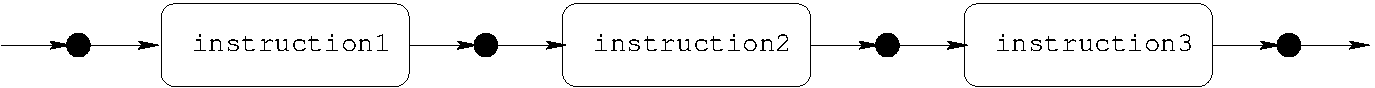
\includegraphics[width=7.5cm]{uml0.pdf}}
\end{fig}

\begin{fig}[Définition de l'académie (6)]\label{fig:dico6}
\mbox{}\\
{\bf ALTERNATIVE} n. f. XVe siècle, comme terme de droit ecclésiastique ; 
XVIIe siècle, au sens moderne. Forme féminine substantivée d'alternatif.
Choix nécessaire entre deux propositions, deux attitudes dont l'une exclut l'autre. 
\end{fig}}
Sauf mention explicite, les instructions d'un algorithme s'exécutent 
les unes après les autres, dans l'ordre où elles ont été écrites.
Le « chemin » suivi à travers un algorithme est appelé le flux d'instructions
(figure \ref{fig:flux}), 
et les constructions qui le modifient sont appelées des instructions de contrôle de flux.
On exécute normalement les instructions de la première à la dernière, sauf lorsqu'on rencontre
une instruction de contrôle de flux : de telles instructions vont permettre de suivre 
différents chemins suivant les circonstances.
C'est en particulier le cas de l'instruction conditionnelle qui n'exécute une instruction
que sous certaines conditions préalables. Nous distinguerons ici 3 variantes d'instructions conditionnelles 
(figure \ref{fig:dico6}) : 
\marginpar{\footnotesize\em
\begin{rem}A propos des instructions conditionnelles, on parle souvent des instructions 
« {\tt if} » dans le jargon des informaticiens.
\end{rem}

\begin{rem}{\tt elif ...} et la contraction de {\tt else: if ...}.\end{rem}
}
\index{test}\index{alternative|see{test}}
$$\begin{tabular}{|l|l|}
\hline
\multicolumn{2}{|c|}{Instructions conditionnelles}\\
\hline
test simple         & {\begin{minipage}[t]{6cm}\tt if condition : blocIf \\ \mbox{} \end{minipage}} \\
\hline
alternative simple   & {\begin{minipage}[t]{6cm}\tt if condition : blocIf\\else: blocElse \\ \mbox{} \end{minipage}} \\
\hline
alternative multiple & {\begin{minipage}[t]{6cm}\tt if condition : blocIf\\elif condition1: blocElif1\\elif
condition2: blocElif2\\ \ldots \\else: blocElse \\ \mbox{} \end{minipage}}\\
\hline
\end{tabular}$$
où {\tt if}, {\tt else} et {\tt elif} sont des mots réservés, {\tt condition} une expression
booléenne (à valeur {\tt True} ou {\tt False}) et {\tt bloc...} un bloc d'instructions.


%-------------------------------------------------------------------------
\subsection{Tests simples}\label{sub:cond}
%-------------------------------------------------------------------------
L'instruction « {\tt if} » sous sa forme la plus simple (figure \ref{fig:test})
permet de tester la validité d'une condition.
\index{instruction!test simple}\index{if1@{{\tt if}}}
Si la condition est vraie,
alors le bloc d'instructions {\tt blocIf} après le « {\tt :} » est exécuté. 
Si la condition est fausse, on passe à l'instruction suivante dans le flux 
d'instructions. 
\marginpar{\footnotesize\em\vspace*{-2cm}
\begin{fig}[Le test simple]\label{fig:test}\tt 
if condition : blocIf
\end{fig}
\index{langage!{{\sc Python}}!opérateurs}
\begin{fig}[Principaux opérateurs \python]\label{fig:operateur}
\begin{description}
\item[Opérateurs logiques :] {\tt not a}, {\tt a and b}, {\tt a or b}
\item[Opérateurs de comparaison :] {\tt x == y}, {\tt x != y},\\{\tt x < y}, {\tt x <= y}, 
	{\tt x > y}, {\tt x >= y}
\item[Opérateurs arithmétiques :] {\tt +x}, {\tt -x}, {\tt x + y}, \\{\tt x - y}, {\tt x * y}, 
	{\tt x / y}, {\tt x \% y}, {\tt x**y}
\end{description}
\end{fig}
\begin{td}[Opérateurs booléens dérivés (1)]\label{td:booleens1}\index[td]{opérateurs booléens dérivés}
En utilisant les opérateurs booléens de base ({\tt not}, {\tt and} et {\tt or}),
écrire un algorithme qui affecte successivement à une variable {\tt s} 
le résultat des opérations booléennes suivantes :
ou exclusif ({\em xor}, $a \oplus b$), 
non ou ({\em nor}, $\overline{a+b}$), 
non et ({\em nand}, $\overline{a\cdot b}$), 
implication ($a \Rightarrow b$) et  
équivalence ($a \Leftrightarrow b$).
\end{td}

\index[algo]{circuits logiques}
\begin{td}[Circuit logique (1)]\label{td:circuits}\index[td]{circuits logiques}
Donner les séquences d'affectations permettant de calculer la sortie $s$
du circuit logique suivant en fonction de ses entrées $a$, $b$ et $c$.
$$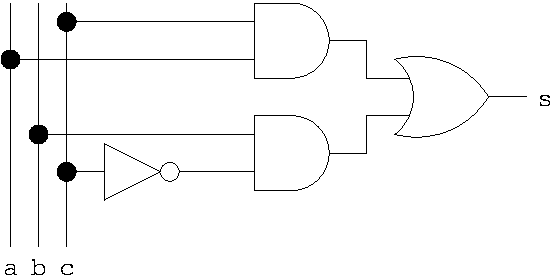
\includegraphics[width=5cm]{mux1.pdf}$$
\end{td}}

\begin{defin}[test simple]\index[def]{test simple}\index{test!test simple}
Le test simple est une instruction de contrôle du flux d'instructions 
qui permet d'exécuter une instruction sous condition préalable.
\end{defin}

La condition évaluée après l'instruction « {\tt if} »  est donc une 
expression booléenne qui prend soit la valeur {\tt False} (faux) soit la valeur 
{\tt True} (vrai). Elle peut contenir les opérateurs de comparaison suivants :
$$\begin{tabular}{l@{\tt\hspace*{1cm}\# }l}
\tt x == y                &  {\tt x} est   égal à {\tt y} \\
\tt x != y                &  {\tt x} est   différent de {\tt y} \\
\tt x > y                 &  {\tt x} est   plus grand que {\tt y} \\
\tt x < y                 &  {\tt x} est   plus petit que {\tt y} \\
\tt x >= y                &  {\tt x} est   plus grand que, ou égal à {\tt y} \\
\tt x <= y                &  {\tt x} est   plus petit que, ou égal à {\tt y}
\end{tabular}$$
Mais certains problèmes exigent parfois de formuler des conditions qui ne peuvent pas être exprimées 
sous la forme d'une simple comparaison. Par exemple, la condition $x \in [0,1[$ s'exprime 
par la combinaison de deux conditions $x \geq 0$ et $x < 1$ qui doivent être vérifiées en même temps. 
Pour combiner ces conditions, on utilise les opérateurs logiques {\tt not}, {\tt and} et {\tt or}
(figure \ref{fig:operateur}). Ainsi la condition $x \in [0,1[$ pourra s'écrire en \python\ :
{\tt (x >= 0) and (x < 1)}.
\exo{td:booleens1}

Le tableau ci-dessous donne les tables de vérité des opérateurs {\tt not}, {\tt or} et {\tt and},
leur représenta\-tion graphique traditionnelle ainsi que leurs principales propriétés. 
\exo{td:circuits}

\index{opérateurs booléens}
$$\begin{tabular}{|c|c|c|}
\hline
négation & disjonction & conjonction \\
\hline
\tt not a & \tt a or b & \tt a and b\\
$\begin{array}{|c|c|}
\hline
a & {\overline{a}}\\
\hline
0 & 1\\
1 & 0\\
\hline
\end{array}$ &
$\begin{array}{|c|c|c|}
\hline
a & b & {a+b}\\
\hline
0 & 0 & 0\\
0 & 1 & 1\\
1 & 0 & 1\\
1 & 1 & 1\\
\hline
\end{array}$ &
$\begin{array}{|c|c|c|}
\hline
a & b & {a\cdot b}\\
\hline
0 & 0 & 0\\
0 & 1 & 0\\
1 & 0 & 0\\
1 & 1 & 1\\
\hline
\end{array}$ \\
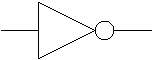
\includegraphics[height=0.75cm]{non.pdf} & 
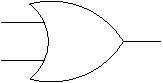
\includegraphics[height=0.75cm]{ou.pdf}  &
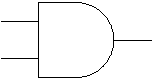
\includegraphics[height=0.75cm]{et.pdf}  \\
\hline
 & \tt not (a or b) & \tt not (a and b) \\
 & 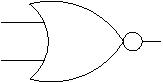
\includegraphics[height=0.75cm]{nonOu.pdf} & 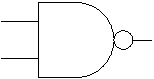
\includegraphics[height=0.75cm]{nonEt.pdf}\\
\hline
\end{tabular}
\hfill
\begin{tabular}{ll}
\multicolumn{2}{l}{$\forall a, b, c \in \{0;1\}$ :}\\
\makebox[0.5cm]{} & {$a + 0 = a$} \hspace*{5mm} {$a \cdot 1 = a$}\\
 & {$a + 1 = 1$} \hspace*{5mm} {$a \cdot 0 = 0$}\\
 & {$a + a = a$} \hspace*{5mm} {$a \cdot a = a$}\\
 & {$a + \overline{a} = 1$} \hspace*{5mm} {$a \cdot \overline{a} = 0$}\\
 & {$a + (a \cdot b) = a$} \hspace*{5mm} {$a \cdot (a + b) = a$}\\
 & {$\overline{\overline{a}}  = a$} \hspace*{5mm} $\overline{a + b} = \overline{a} \cdot \overline{b}$ \hspace*{5mm} $\overline{a\cdot b} = \overline{a} + \overline{b}$\\
 & {$(a+b) = (b+a)$} \hspace*{5mm}  {$(a \cdot b) = (b \cdot a)$} \\
 & {$(a+b)+c = a+(b+c)$} \\ 
 & {$(a\cdot b)\cdot c = a\cdot (b\cdot c)$} \\
 & {$a + (b \cdot c) = (a+b) \cdot (a+c)$} \\ 
 & {$a \cdot (b+ c) = (a \cdot b)+(a\cdot c)$} 
\end{tabular}$$
\exo{td:prop}
\marginpar{\footnotesize\em
\begin{td}[Lois de De Morgan]\label{td:prop}\index{{{\sc De Morgan}}}\index[td]{lois de {{\sc De Morgan}}}
Démontrer à l'aide des tables de vérité les lois de De Morgan 
$\forall a, b \in \{0;1\}$ :
\begin{enumerate}
\item {$\overline{(a+b)} = \overline{a} \cdot \overline{b}$} 
\item {$\overline{(a \cdot b)} = \overline{a} + \overline{b}$}
\end{enumerate}
\end{td}
\begin{fig}[L'alternative simple]\label{fig:alternative}\tt 
if condition : blocIf\\
else: blocElse
\end{fig}

\begin{rem}Le test simple (figure \ref{fig:test} page \pageref{fig:test}) est équivalent 
à une alternative simple où on explicite le fait de ne rien faire (instruction {\tt pass})
dans le bloc d'instructions associé au {\tt else}:\\
{\tt
\mbox{}\ \ if condition : bloc\\
\mbox{}\ \ else: pass}\\
\mbox{}\hfill voir également le TD \ref{td:reciproque} page \pageref{td:reciproque}.
\end{rem}}

%-------------------------------------------------------------------------
\subsection{Alternatives simples}\label{sub:alternative}
%-------------------------------------------------------------------------
\begin{ex}[Extrait d'un dialogue entre un conducteur égaré et un piéton]\label{ex:chemin}
\begin{itemize}
\item Pourriez-vous m'indiquer le chemin de la gare, s'il vous plait ?
\item Oui bien sûr : vous allez tout droit jusqu'au prochain carrefour.
	Si la rue à droite est autorisée à la circulation --- hier elle était en travaux --- 
	alors prenez la et ensuite c'est
	la deuxième à gauche et vous verrez la gare. Sinon, au carrefour, vous allez tout droit 
	et vous prenez la
	première à droite, puis encore la première à droite et vous y êtes.
\item Merci.
\end{itemize}
\end{ex}
\noindent L'algorithme décrit par le piéton propose une alternative entre deux solutions.
Le conducteur égaré devra tester si la rue est en travaux avant de prendre la décision 
d'aller à droite au carrefour ou de continuer tout droit. En algorithmique, un tel
choix est proposé par l'alternative simple, instruction conditionnelle
dite « {\tt if} \ldots\ {\tt else} ».\index{if2@{{\tt if\ \ldots\ else}}}

L'instruction « {\tt if} \ldots\ {\tt else} » teste une condition (figure \ref{fig:alternative}). 
\index{instruction!alternative simple}
Si la condition
est vraie, alors le bloc d'instructions {\tt blocIf} après le « {\tt :} » est exécuté.
Si la condition est fausse, c'est le bloc d'instructions {\tt blocElse} après le « {\tt else:} » 
(sinon) qui est exécuté. Seul l'un des 2 blocs est donc exécuté.

\begin{defin}[alternative simple]\index[def]{alternative simple}\index{test!alternative simple}
L'alternative simple est une instruction de contrôle du flux d'instructions 
qui permet de choisir entre deux instructions selon qu'une condition est vérifiée ou non.
\end{defin}
\marginpar{\footnotesize\em
\begin{td}[Maximum de 2 nombres]\label{td:max}\index[algo]{maximum de 2 nombres}\index[td]{maximum de 2 nombres}
Ecrire un algorithme qui détermine le maximum $m$ de 2 nombres $x$ et $y$.
\end{td}
\begin{td}[Fonction « porte »]\label{td:porte}\index[td]{fonction porte}
Proposer une autre alternative simple pour calculer la fonction « porte » de
l'exemple \ref{ex:porte} ci-contre. 
\end{td}
\begin{fig}[Aiguillage « {\tt if ... else} »]\label{fig:uml1}
{\tt 
if condition : blocIf\\
else: blocElse}
$${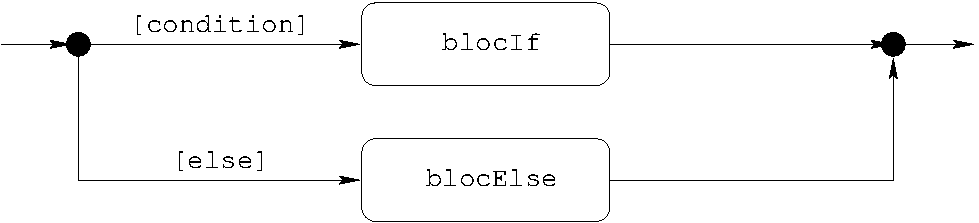
\includegraphics[width=7.5cm]{uml1.pdf}}$$
L'étiquette {\tt [condition]} signifie qu'on passe par la voie correspondante 
si la condition est vérifiée ({\tt True}), sinon on passe par la voie étiquettée
{\tt [else]}.
\end{fig}
}

\begin{ex}[Valeur absolue d'un nombre]\index[algo]{valeur absolue}
L'algorithme qui détermine la valeur absolue $y$ d'un nombre $x$ peut s'écrire de la manière suivante :\\
{\footnotesize\tt
\mbox{}\ \ if x < 0: y = -x\\
\mbox{}\ \ else: y = x
}
\end{ex}
\noindent On commence par tester le signe de $x$ ({\tt if x < 0}), si $x < 0$, alors la valeur absolue $y$
vaut $-x$ ({\tt : y = -x}) sinon ($x \geq 0$) elle vaut $x$ ({\tt else: y = x}).
\exo{td:max}

\begin{ex}[Fonction « porte »]\label{ex:porte}\mbox{}\\
\begin{minipage}{11cm}
On considère la fonction « porte » $f$ dont le graphe est donné ci-contre.
L'alternative suivante permet de calculer $y = f(x)$ :\\
{\footnotesize\tt
\mbox{}\ \ if x < -1 or x > 2: y = 0\\
\mbox{}\ \ else: y = 2
}\exo{td:porte}
\end{minipage}
\hfill
\begin{minipage}{4cm}
\centerline{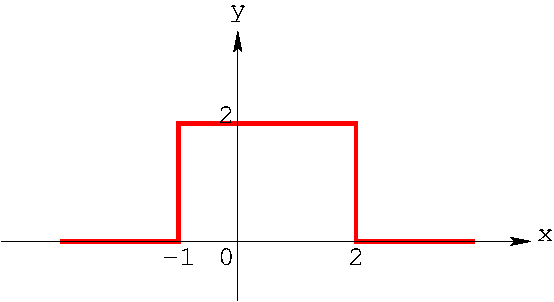
\includegraphics[width=4cm]{porte.pdf}}
\end{minipage}
\end{ex}
Les exemples \ref{ex:chemin} et \ref{ex:porte} précédents nous montrent
qu'une alternative se comporte comme un aiguillage de chemin de fer 
dans le flux d'instructions (figure \ref{fig:uml1}). 
Un « {\tt if ... else} » ouvre  deux voies correspondant à deux traitements différents, 
et seule une de ces voies sera empruntée (un seul des deux traitements est
exécuté). Mais il y a des situations où deux voies ne suffisent pas : on utilise
alors des alternatives simples en cascade (ou alternatives multiples). 

%-------------------------------------------------------------------------
\subsection{Alternatives multiples}\label{sub:alternatives}
%-------------------------------------------------------------------------
\begin{ex}[Etat de l'eau]
A pression ambiante, l'eau est sous forme de glace si la température
est inférieure à $0^\circ C$, sous forme de liquide si la température
est comprise entre $0^\circ C$ et $100^\circ C$ et sous forme de vapeur
au-delà de $100^\circ C$.
\end{ex}
\marginpar{\footnotesize\em
\begin{fig}[« {\tt if ... else} » imbriqués]\label{fig:uml2}
{\tt 
if condition1 : blocIf1\\
else: \\
\mbox{}\ \ \ \ if condition2 : blocIf2\\
\mbox{}\ \ \ \ else: blocElse}
$${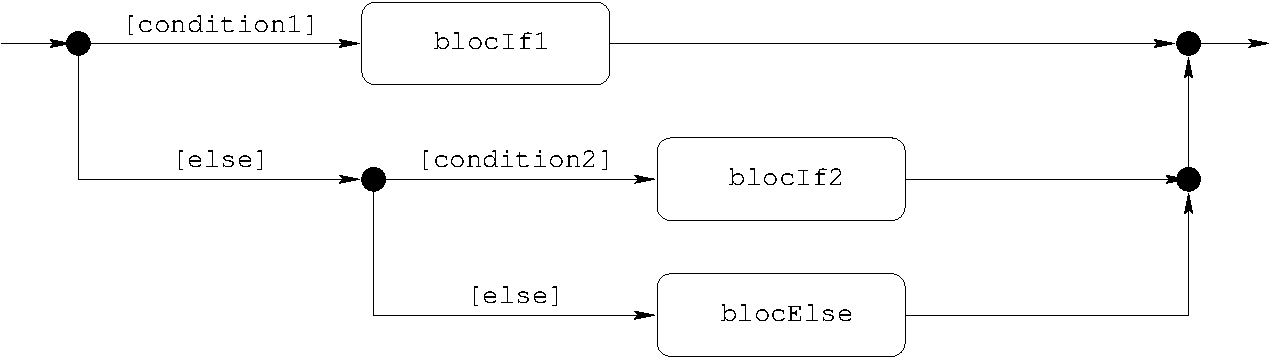
\includegraphics[width=7.5cm]{uml2.pdf}}$$
\end{fig}
\begin{td}[Ouverture d'un guichet]\label{td:guichet}\index[td]{ouverture d'un guichet}
A l'aide d'alternatives simples imbriquées, écrire un algorithme qui détermine 
si un guichet est {\tt 'ouvert'} ou 
{\tt 'fermé'} selon les jours de la semaine ({\tt 'lundi'}, {\tt 'mardi'},
\ldots\ ,{\tt 'dimanche'}) et l'heure de la journée (entre 0h et 24h).
Le guichet est ouvert tous les jours de 8h à 13h et de 14h à 17h 
sauf le samedi après-midi et toute la journée du dimanche.
\end{td}
}
\noindent Un algorithme qui devrait déterminer l'état de l'eau en fonction de
la température doit pouvoir choisir entre trois réponses possibles :
solide, liquide ou vapeur. Une première version de cet algorithme utilise
3 tests simples :\\
{\footnotesize\tt
\mbox{}\ \ if t < 0 : eau = 'glace'\\
\mbox{}\ \ if t >= 0 and t <= 100 : eau = 'liquide'\\
\mbox{}\ \ if t > 100 : eau = 'vapeur'\\
}
Cet algorithme est correct mais va évaluer les 3 conditions 
qui portent sur la même variable
{\tt t} et qui sont exclusives les unes des autres; en effet, si {\tt (t < 0)}, alors
on ne peut pas avoir {\tt (t >= 0 and t <= 100)} ni {\tt (t > 100)}. 
Il est donc inutile d'évaluer les 2 dernières conditions si la première 
est vérifiée, ou d'évaluer la dernière condition si la deuxième est vérifiée.
On préfère donc imbriquer les tests de la manière suivante :\\
{\footnotesize\tt
\mbox{}\ \ if t < 0 : eau = 'glace'\\
\mbox{}\ \ else :\\
\mbox{}\ \ \ \ \ \ if t <= 100 : eau = 'liquide'\\
\mbox{}\ \ \ \ \ \ else: eau = 'vapeur'
}\exo{td:guichet}\\
On commence par évaluer la première condition {\tt (t < 0)}. Si la condition est vérifiée,
on exécute l'affectation {\tt eau = 'glace'}; sinon {\tt (t >= 0)}, on évalue la deuxième 
condition {\tt (t <= 100)} qui en fait est équivalente à {\tt (t >= 0) and (t <= 100)}. 
Si la condition est vérifiée, on exécute l'affectation {\tt eau = 'liquide'};
sinon {\tt (t > 100)}, on exécute l'affectation {\tt eau = 'vapeur'}.
La figure \ref{fig:uml2} illustre le contrôle du flux d'instructions lors de deux
« {\tt if \ldots\ else} » imbriqués : il s'agit de deux aiguillages en cascade.
Afin de simplifier l'écriture des tests imbriqués, on peut contracter le « {\tt else: if} »
en {\tt elif} et obtenir une version plus compacte de l'algorithme, 
strictement équivalente à la version précédente :\\
{\footnotesize\tt
\mbox{}\ \ if t < 0 : eau = 'glace'\\
\mbox{}\ \ elif t <= 100 : eau = 'liquide'\\
\mbox{}\ \ else: eau = 'vapeur'\\
}

\marginpar{\footnotesize\em\vspace*{-1cm}
\begin{fig}[L'alternative multiple]\label{fig:alternatives}
{\tt 
if condition : blocIf\\
elif condition1 : blocElif1\\
elif condition2 : blocElif2\\
\ldots\\
else: blocElse}
$$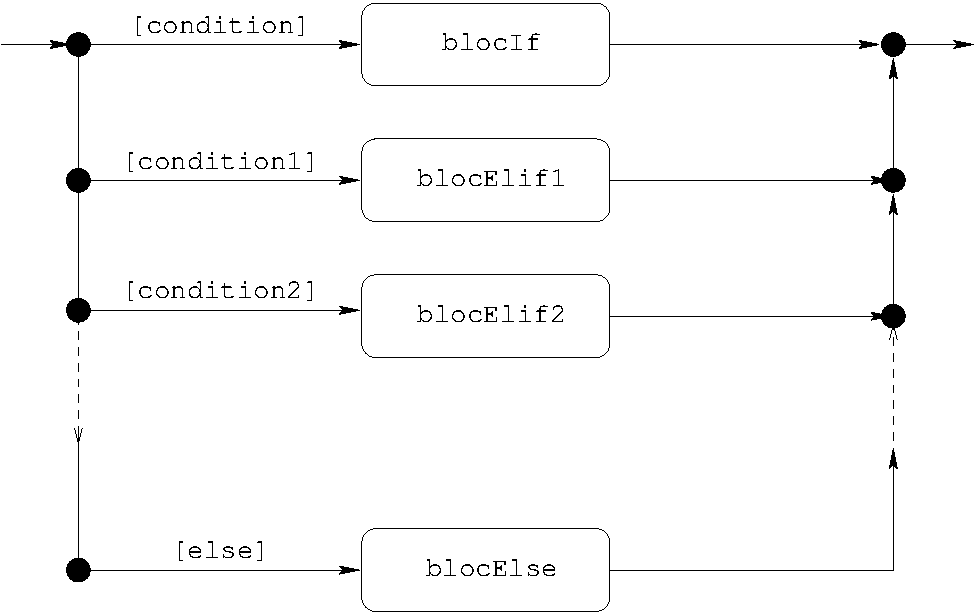
\includegraphics[width=7.5cm]{uml3.pdf}$$
L'alternative multiple ci-dessus est équivalente
à un ensemble d'alternatives simples imbriquées :\\
{\tt
if condition : blocIf\\
else:\\
\mbox{}\ \ \ \ if condition1 : blocElif1\\
\mbox{}\ \ \ \ else:\\
\mbox{}\ \ \ \ \ \ \ \ if condition2 : blocElif2\\
\mbox{}\ \ \ \ \ \ \ \ else:\\
\mbox{}\ \ \ \ \ \ \ \ \ $\ddots$\\
\mbox{}\ \ \ \ \ \ \ \ \ \ \ \ \ else: blocElse}
\end{fig}
}
\index{if3@{{\tt if\ \ldots\ elif\ \ldots\ else}}}\index{instruction!alternative multiple}
L'instruction « {\tt if} \ldots\ {\tt elif} » teste une première condition (figure \ref{fig:alternatives}). 
Si cette condition est vraie, alors le bloc d'instructions {\tt blocIf} 
est exécuté. Si la première condition est fausse, on teste la deuxième ({\tt condition1}).
Si la deuxième condition est vérifiée, c'est le bloc d'instructions {\tt blocElif1} après le premier « {\tt elif:} » 
(sinon-si) qui est exécuté; sinon on teste la condition suivante ({\tt condition2}).
Si elle est vérifiée, c'est le bloc d'instructions {\tt blocElif2} après le deuxième « {\tt elif:} » 
qui est exécuté et ainsi de suite. Si aucune des conditions n'est vérifiée, c'est le bloc d'instructions
{\tt blocElse} qui est exécuté. Dans tous les cas, un seul des blocs est donc exécuté.

\begin{defin}[alternative multiple]\index[def]{alternative multiple}\index{test!alternative multiple}
L'alternative multiple est une instruction de contrôle du flux d'instructions 
qui permet de choisir entre plusieurs instructions en cascadant des alternatives simples.
\end{defin}


\begin{ex}[Mentions du baccalauréat]
Au baccalauréat, la mention associée à une note sur 20 est
	{\tt 'très bien'} pour les notes supérieures ou égales à 16,
	{\tt 'bien'} pour les notes comprises entre 14 inclus et 16 exclu, 
	{\tt 'assez bien'} pour les notes comprises entre 12 inclus et 14 exclu, 
	{\tt 'passable'} pour les notes comprises entre 10 inclus et 12 exclu et
	{\tt 'insuffisant'} pour les notes strictement inférieures à 10.
\end{ex}
\marginpar{\em\footnotesize
\begin{td}[Catégorie sportive]\label{td:categorie}\index[td]{catégorie sportive}
Ecrire un algorithme qui détermine la catégorie sportive d'un enfant selon
son âge : 
	\begin{itemize}
	\item Poussin de 6 à 7 ans,
	\item Pupille de 8 à 9 ans,
	\item Minime de 10 à 11 ans,
	\item Cadet de 12 ans à 14 ans.
	\end{itemize}
\end{td}}
\noindent On peut utiliser une alternative multiple pour déterminer la mention 
au bac en fonction de la note :\\
{\footnotesize\tt
\mbox{}\ \ if note < 10: mention = 'insuffisant'\\
\mbox{}\ \ elif note < 12: mention = 'passable'\\
\mbox{}\ \ elif note < 14: mention = 'assez bien'\\
\mbox{}\ \ elif note < 16: mention = 'bien'\\
\mbox{}\ \ else: mention = 'très bien'\\
}
\exo{td:categorie}


%-------------------------------------------------------------------------
\section{Boucles}\label{boucles}
%-------------------------------------------------------------------------
\index{itération|see{boucle}}\index{répétition|see{boucle}}
\begin{ex}[Un calcul de pgcd (2)]\label{ex:pgcd2}\index[algo]{algorithme d'{{\sc Euclide}}}
Le plus grand commun diviseur de 2 entiers $a$ et $b$ peut se calculer en appliquant
la relation de récurrence ${\rm pgcd}(a,b) = {\rm pgcd}(b,a\mbox{\tt\%}b)$ jusqu'à ce que le reste
($a\%b$) soit nul.\\
Dans l'exemple \ref{ex:pgcd1} page \pageref{ex:pgcd1}, 
pour calculer le pgcd de $a=12$ et de $b=18$, on appliquait 3 fois de suite
cette relation :
${\rm pgcd}(12,18) = {\rm pgcd}(18,12) = {\rm pgcd}(12,6) = {\rm pgcd}(6,0) = 6$. 
L'algorithme correspondant faisait donc apparaître 3 fois de suite les mêmes instructions 
après l'initialisation des variables $a$ et $b$ :\\
{\tt
\mbox{}\ \ r = a\%b\\
\mbox{}\ \ a = b\\
\mbox{}\ \ b = r}\\
Si nous voulons maintenant calculer le pgcd de $44$ et $5648$, 
il nous faudra répéter 5 fois la même séquence d'instructions pour trouver
que ${\rm pgcd}(44,5648) = 4$. 
\end{ex}
\noindent Ce nouvel exemple de calcul de pgcd soulève au moins 2 questions :
\begin{enumerate}
\item Comment éviter de répéter explicitement plusieurs fois de suite la même 
	séquence d'instructions ? 
\item Comment éviter de savoir à l'avance combien de fois il faut répéter
	la séquence pour obtenir le bon résultat ? 
\end{enumerate}
\marginpar{\footnotesize\em
\begin{fig}[Définition de l'académie (7)]\label{fig:dico7}
{\bf ITÉRATION} n. f. XVe siècle. Emprunté du latin iteratio, « répétition, redite ».
Répétition. MATH. Répétition d'un calcul avec modification de la variable, 
qui permet d'obtenir par approximations successives un résultat satisfaisant.
\end{fig}

\begin{rem}
A propos des instructions itératives,
on parle souvent des boucles « {\tt while} » ou des boucles « {\tt for} » 
dans le jargon des informaticiens.
\end{rem}
}
De nouvelles instructions de contrôle de flux sont introduites pour répondre
à ces questions : les instructions itératives. On parle également de boucles, de répétitions
ou encore d'itérations (figure \ref{fig:dico7}).
Nous distinguerons 2 variantes d'instructions itératives :
$$\begin{tabular}{|l|l|}
\hline
\multicolumn{2}{|c|}{Instructions itératives}\\
\hline
itération conditionnelle & {\begin{minipage}[t]{6cm}\tt while condition : blocWhile \\ \mbox{} \end{minipage}} \\
\hline
parcours de séquence & {\begin{minipage}[t]{7cm}\tt for element in sequence : blocFor \\ \mbox{} \end{minipage}} \\
\hline
\end{tabular}$$
où {\tt while}, {\tt for} et {\tt in} sont des mots réservés, {\tt condition} une expression
booléenne (à valeur {\tt True} ou {\tt False}), {\tt element} un élément de la séquence {\tt sequence}
et {\tt bloc...} un bloc d'instructions.


%-------------------------------------------------------------------------
\subsection{Itération conditionnelle}
%-------------------------------------------------------------------------
\marginpar{\footnotesize\em
\begin{fig}[Boucle {\tt while}]\label{fig:while}
{\tt while condition : blocWhile}
$$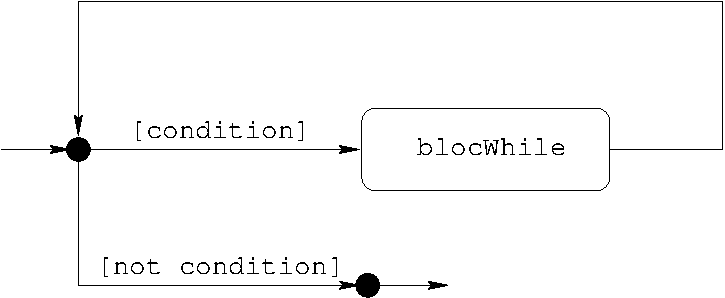
\includegraphics[width=7.5cm]{uml4.pdf}$$
\end{fig}}
L'instruction « {\tt while} » \index{while@{{\tt while}}} permet de répéter plusieurs fois une même instruction 
(figure \ref{fig:while}) : le bloc d'instructions {\tt blocWhile} est exécuté tant que
({\em while}) la condition est vérifiée. On arrête dès que la condition est fausse; 
on dit alors qu'on « sort » de la boucle. 

On commence par tester la condition; si elle
est vérifiée, on exécute le bloc d'instructions {\tt blocWhile} 
(encore appelé le «~corps~» de la boucle) puis on reteste la condition : 
la condition est ainsi évaluée avant chaque exécution du corps 
de la boucle; si la condition est à nouveau vérifiée on réexécute le bloc 
d'instructions {\tt blocWhile} (on dit qu'on « repasse » dans la boucle)
et ainsi de suite jusqu'à ce que la condition devienne fausse, 
auquel cas on « sort » de la boucle.

\begin{defin}[itération conditionnelle]\index[def]{itération conditionnelle}\index{boucle!itération conditionnelle}
L'itération conditionnelle est une instruction de contrôle du flux d'instructions
qui permet sous condition préalable de répéter zéro ou plusieurs fois la même instruction.
\end{defin}

\begin{ex}[Table de multiplication]\label{ex:table}\index[algo]{tables de multiplication}
On cherche à écrire un algorithme qui affiche la table de multiplication
d'un nombre $n$ quelconque.\\
Exemple : $n = 9 \rightarrow\ $
\begin{py}{3cm}
\begin{verbatim}
1 * 9 = 9
2 * 9 = 18
3 * 9 = 27
4 * 9 = 36
5 * 9 = 45
6 * 9 = 54
7 * 9 = 63
8 * 9 = 72
9 * 9 = 81
\end{verbatim}
\end{py}
\hfill
\begin{minipage}[t]{8cm}
L'affichage ci-contre est obtenu par l'algorithme suivant :
\begin{py}{5cm}
\begin{verbatim}
n = 9
i = 1
while i < 10:
    print(i, '*', n, '=', i*n)
    i = i + 1
\end{verbatim}
\end{py}
\end{minipage}
\end{ex}

\noindent L'algorithme précédent commence par initialiser {\tt n} et le multiplicateur {\tt i}.
Ensuite, puisque {\tt i < 10}, on rentre dans la boucle; la première instruction
{\tt print} affiche successivement la valeur de {\tt i}, une {\tt *}, 
la valeur de {\tt n}, le signe {\tt =} puis la valeur du produit {\tt i*n}, 
soit au premier passage : {\tt 1 * 9 = 9}. L'instruction suivante incrémente {\tt i} qui devient
ainsi égal à {\tt 2} ({\tt 1 + 1}). Les deux instructions du corps de la boucle {\tt while} ayant 
été exécutées, on reteste la condition {\tt i < 10}; elle est à nouveau vérifiée puisque {\tt i}
vaut maintenant {\tt 2}. On repasse alors dans la boucle où on affiche {\tt 2 * 9 = 18} et où on
incrémente {\tt i} qui vaut maintenant {\tt 3} ({\tt 2 + 1}). On réitère ces opérations jusqu'à 
ce que {\tt i} soit égal à {\tt 10} ({\tt 9 + 1}); entre-temps les 7 autres lignes de la table de 
multiplication par {\tt 9} ont été affichées. Lorsque {\tt i} vaut {\tt 10}, la condition {\tt i < 10}
n'est plus vérifiée et on « sort » de la boucle {\tt while}.
\exo{td:etoile}

\marginpar{\footnotesize\em
\begin{td}[Dessin d'étoiles (1)]\label{td:etoile}\index[td]{dessin d'étoiles}
Ecrire un algorithme itératif qui affiche les $n$ lignes suivantes (l'exemple
est donné ici pour $n=6$) : \\
\begin{minipage}[t]{2cm}\tt
******\\
*****\\
****\\
***\\
**\\
*
\end{minipage}
\hfill
\begin{minipage}[t]{3cm}
Rappel \python\ : \\
{\tt
\mbox{}\ \ \ \ >>> 5*'r'\\
\mbox{}\ \ \ \ 'rrrrr'\\
\mbox{}\ \ \ \ >>> 2*'to'\\
\mbox{}\ \ \ \ 'toto'
}
\end{minipage}
\end{td}}
Dans une itération conditionnelle, la condition doit évoluer au cours des différents passages
dans la boucle afin de pouvoir sortir de la boucle. C'est le cas de la boucle {\tt while}
de l'exemple \ref{ex:table} ci-dessus; à chaque passage dans la boucle, le
multiplicateur {\tt i} est incrémenté : ainsi, partant de la valeur initiale {\tt i = 1},
{\tt i} deviendra nécessairement égal à {\tt 10} après 9 passages dans la boucle.

En ce qui concerne le nombre de passages dans la boucle, deux cas extrèmes peuvent se produire : 
\begin{itemize}
\item la condition n'est pas vérifiée la première fois : 
	on ne passe alors jamais dans la boucle.
	
	Exemple : 
	\begin{py}{5cm}
	\begin{verbatim}
	x = 4
	y = 0
	while x < 0 : y = y + x
	\end{verbatim}
	\end{py}\hfill
	\begin{minipage}[t]{7.5cm}\footnotesize
	$x$ est positif; la condition $x < 0$ n'est donc pas vérifiée la première
	fois : on ne rentre pas dans la boucle.
	\end{minipage}
\item la condition n'est jamais fausse : on ne sort jamais de la boucle; 
	on dit qu'on a affaire à une boucle « sans fin ».

	Exemple : 
	\begin{py}{5cm}
	\begin{verbatim}
	x = 4
	y = 0
	while y >= 0 : y = y + x
	\end{verbatim}
	\end{py}\hfill
	\begin{minipage}[t]{7.5cm}\footnotesize
	$y$ est initialement nul : on rentre dans la boucle;
	l'instruction du corps de la boucle ne peut qu'incrémenter $y$
	puisque $x$ est positif : $y$ sera donc toujours positif et on 
	ne sortira jamais de la boucle.
	\end{minipage}
\end{itemize}
Le cas de la boucle « sans fin » est évidemment dû le plus souvent à une erreur involontaire
qu'il faut savoir détecter assez vite pour éviter un programme qui « tourne » indéfiniment
sans s'arrêter.

\marginpar{\footnotesize\em
\begin{rem}Une erreur classique de l'apprenti informaticien est de ne pas faire évoluer
la condition d'une boucle {\tt while} : il « tombe » alors dans une boucle « sans fin »
comme dans l'exemple ci-dessous :\\
\begin{minipage}[t]{2.75cm}\tt
\mbox{}\ \ k = 1\\
\mbox{}\ \ p = x\\
\mbox{}\ \ while k <= n:\\
    \mbox{}\ \ \ \ p = p*x
\end{minipage}
\hfill
\begin{minipage}[t]{5cm}
On entre dans la boucle; on calcule la nouvelle valeur de {\tt p}
puis on reteste la condition {\tt k <= n}. Mais entre-temps {\tt k}
n'a pas évolué (il n'a pas été incrémenté) et donc la condition
reste vraie et restera toujours vraie : l'exécution ne sortira plus de la boucle.
\end{minipage}
\end{rem}
}
\begin{ex}[Fonction puissance]\label{ex:puissance}\index[algo]{fonction puissance}
La puissance entière $p$ d'un nombre $x$ est définie par :
$\displaystyle p = x^n = \prod_{k=1}^{n} x = \underbrace{x\cdot x\cdot x\cdots x}_{n\ \rm fois}$ .
\end{ex}
\noindent Pour calculer $p$ « de tête », nous calculons successivement $x$, $x^2$, $x^3$\ldots,
$x^{n-1}$ et $x^n$ en mémorisant à chaque étape la puissance courante $x^k$ et en multipliant
simplement cette puissance par $x$ pour obtenir la puissance immédiatement supérieure $x^{k+1}$.
On s'arrête quand $k = n$ : on a alors le résultat attendu ($p = x^n$).
Cet algorithme peut s'écrire directement :\\
\mbox{}\ \ \begin{py}{3cm}
\begin{verbatim}
k = 1
p = x
while k < n:
    p = p*x
    k = k + 1
\end{verbatim}
\end{py}
\hfill
\begin{minipage}[t]{12cm}\footnotesize
On commence par initialisé l'exposant $k$ à 1 et la puissance $p$ recherchée 
avec la valeur de $x^k = x^1 = x$ ({\tt p = x}). 
Ensuite, pour chaque valeur de $k < n$,
on multiplie la puissance courante $p$ par $x$ ({\tt p*x}) qui devient la nouvelle
puissance courante ({\tt p = p*x}) et on n'oublie pas d'incrémenter l'exposant $k$; ainsi
à la fin de chaque itération, on a toujours $p = x^k\ \forall k \in [1;n]$.
\end{minipage}\\
\exo{td:factorielle}

\marginpar{\footnotesize\em
\begin{td}[Fonction factorielle]\label{td:factorielle}\index[algo]{fonction factorielle}\index[td]{fonction factorielle}
Ecrire un algorithme qui calcule $n! = 1\cdot 2\cdot 3\cdot \ldots \cdot (n-1)\cdot n$.
\end{td}
}
Dans les exemples \ref{ex:table} et \ref{ex:puissance} précédents, on savait à l'avance
combien de fois on devait passer dans les boucles : 9 fois pour afficher une table de 
multiplication et $n$ fois pour calculer $x^n$. Mais ce n'est pas toujours le cas comme 
nous allons le constater dans les deux exemples suivants qui permettent de calculer 
respectivement la fonction exponentielle (exemple \ref{ex:exp} : $e^x$) 
et le pgcd de 2 nombres (exemple \ref{ex:pgcd3} : ${\rm pgcd}(a,b)$).

\begin{ex}[Fonction exponentielle]\label{ex:exp}\index[algo]{développements limités}
La fonction exponentielle peut être calculée en fonction de son d\'eveloppement 
en série entière. 
$$\displaystyle y = \exp(x) \approx \sum_{k=0}^{n} u_k = \sum_{k=0}^{n} \frac{x^{k}}{k!} = 
	1 + x + \frac{x^2}{2} + \ldots + \frac{x^{n}}{n!}$$
Les calculs seront arr\^et\'es lorsque la valeur absolue du terme $u_k$ sera inf\'erieure 
\`a un certain seuil $s$ ($0 < s < 1$). On n'utilisera ni la fonction {\em puissance} ($x^n$) 
ni la fonction {\em facto\-riel\-le} ($n!$) pour effectuer le calcul de $\exp(x)$.
\end{ex}
\noindent Pour ce calcul, on pourrait avoir la même démarche que dans l'exemple \ref{ex:puissance}
de la puissance entière; à savoir, on calcule le premier terme
de la série ($x^0/0! = 1$), on le mémorise dans $y$, on calcule le $2^{\grave eme}$ terme ($x^1/1! = x$) 
et on l'ajoute à la valeur de $y$ précédemment mémorisée ($1 + x$), on calcule le $3^{\grave eme}$ 
terme ($x^2/2! = x^2/2$), on l'ajoute à $y$ ($1 + x + x^2/2$) et ainsi de suite jusqu'à ce que 
le nouveau terme calculé vérifie la 
condition d'arrêt imposée ($|u_k| < s$). Mais chaque évaluation d'un nouveau terme fait intervenir 
{\em a priori} les fonctions puissance ($x^k$) et factorielle ($n!$)\ldots qui sont très coûteuses 
en temps de calcul. On préfère remarquer que le terme $u_{k+1}$ peut s'exprimer simplement en 
fonction du terme précédent $u_k$ selon la relation de récurrence :
$$u_{k+1} = \frac{x^{k+1}}{(k+1)!} = \frac{x}{k+1}\cdot\frac{x^{k}}{k!} = \frac{x}{k+1}u_k$$
et qu'il est donc possible de mémoriser à chaque étape $u_k$ pour calculer le terme suivant 
$u_{k+1}$ sans utiliser ni la fonction puissance, ni la fonction factorielle. 
On obtient alors l'algorithme suivant :\\
\mbox{}\ \ \begin{py}{3cm}
\begin{verbatim}
k = 0
u = 1
y = u
while fabs(u) > s:
    u = u*x/(k+1)
    y = y + u
    k = k + 1
\end{verbatim}
\end{py}
\marginpar{\em\footnotesize
\begin{td}[Fonction sinus]\label{td:sinus}\index[algo]{développements limités}\index[td]{fonction sinus}
Ecrire un algorithme qui calcule de manière itérative la fonction sinus
en fonction de son d\'eveloppement en série entière.\\
$\displaystyle\sin(x) \approx \sum_{k=0}^{n} u_k = \sum_{k=0}^{n} (-1)^k\frac{x^{2k+1}}{(2k+1)!}\\
\mbox{}\hfill = x - \frac{x^3}{6} + \frac{x^5}{120} + \ldots + (-1)^n\frac{x^{2n+1}}{(2n+1)!}$\\
Les calculs seront arr\^et\'es lorsque la valeur absolue du terme $u_k$ sera 
inf\'erieure \`a un certain seuil $s$ ($0 < s < 1$). On n'utilisera ni la fonction 
{\em puissance} ($x^n$) ni la fonction {\em facto\-riel\-le} ($n!$) pour effectuer
le calcul de $\sin(x)$.
\end{td}}
\hfill
\begin{minipage}[t]{12cm}\footnotesize
On initialise l'indice {\tt k} à {\tt 0}, le terme {\tt u} (= $u_k$) à la valeur du premier
terme de la série ($x^0/0! = 1$) et {\tt y} à ce premier terme ({\tt y = u}). Puis, tant que la valeur absolue
de $u_k$ ({\tt fabs(u)}) est supérieure au seuil {\tt s}, on calcule le terme suivant $u_{k+1}$ en
utilisant la relation de récurrence obtenue ci-dessus ({\tt u = u*x/(k+1)}) : le nouveau terme $u_{k+1}$
est égal à l'ancien terme $u_k$ multiplié par $x/(k+1)$; on ajoute $u_{k+1}$ à la somme courante $y$
({\tt y = y + u}) et on recommence sans oublier d'incrémenter {\tt k} ({\tt k = k + 1}). 
A la fin de chaque itération, on a toujours $\displaystyle y = \sum_{i=0}^{k} u_i$.
\end{minipage}\\
Ici, on connait la condition d'arrêt de la boucle ($|u_k| < s$) mais on ne sait pas {\em a priori} 
combien de fois on passera dans la boucle : on ne connait pas l'ordre $n$ pour lequel on arrêtera le
développement de la série entière.
\exo{td:sinus}


\begin{ex}[Un calcul de pgcd (3)]\label{ex:pgcd3}
\index[algo]{algorithme d'{{\sc Euclide}}}\mbox{}
On considère à nouveau la relation de récurrence qui caractérise
le pgcd de 2 entiers $a$ et $b$ (voir exemples \ref{ex:pgcd1} et \ref{ex:pgcd2}) : 
${\rm pgcd}(a,b) = {\rm pgcd}(b,a\mbox{\tt\%}b)$. Cette relation nous dit de remplacer
$a$ par $b$ et $b$ par $r = a\%b$ autant de fois que possible jusqu'à ce que le reste
soit nul (${\rm pgcd}(a,0) = a$). Ce qui conduit à l'algorithme suivant :\\
\mbox{}\ \ \begin{py}{2cm}
\begin{verbatim}
while b != 0:
    r = a%b
    a = b
    b = r
\end{verbatim}
\end{py}
\hfill
\begin{minipage}[t]{12cm}\footnotesize
A la fin de chaque passage dans le corps de la boucle, $a$, $b$ et $r$ prennent
successivement les valeurs suivantes ($r$ n'est pas connu avant la boucle) :
$$\begin{tabular}{|l|c|c|c|}
\cline{2-4}
\multicolumn{1}{l|}{}                 &$a$ & $b$ & $r$\\
\hline
avant la boucle  & 12 & 18 & ?\\
\hline
$1^{er}$ passage & 18 & 12 & 12 \\
$2^{\grave eme}$ passage & 12 & 6 & 6\\
$3^{\grave eme}$ passage & 6 & 0 & 0\\
\hline
après la boucle  & 6  & 0 & 0\\
\hline
\end{tabular}$$
\end{minipage}
\end{ex}

\noindent Cet algorithme de calcul de pgcd est connu sous le nom 
d'algorithme d'Euclide (figure \ref{fig:euclide}) et fait partie des grands classiques 
de l'algorithmique.
\exo{td:euclide}\\
Là encore, la condition d'arrêt est connue ($b \neq 0$) mais pas le nombre de passages dans la boucle.
\exo{td:division}
\marginpar{\footnotesize\em
\begin{fig}[Euclide]\label{fig:euclide}
Euclide (né vers -325, mort vers -265) était un mathématicien de la Grèce antique, auteur des «~Éléments~», 
qui sont considérés comme l'un des textes fondateurs des mathématiques modernes.
En particulier, le livre 7 traite de l'arithmétique : il y définit la division 
que l'on appelle division euclidienne et un algorithme pour calculer le plus grand commun diviseur 
de deux nombres, connu sous le nom d'algorithme d'Euclide.
\end{fig}

\begin{td}[Algorithme d'Euclide]\label{td:euclide}\index[td]{algorithme d'{{\sc Euclide}}}
Dans la tradition grecque, en comprenant un nombre entier comme une longueur, 
un couple d'entiers comme un rectangle, leur pgcd est la taille du plus grand 
carré permettant de carreler ce rectangle. L'algorithme décompose ce rectangle 
en carrés, de plus en plus petits, par divisions euclidiennes successives, 
de la longueur par la largeur, puis de la largeur par le reste, 
jusqu'à un reste nul.\\
Faire la construction géométrique «~à la grecque antique~» qui permet de déterminer 
le pgcd $d$ de $a=21$ et $b=15$ ($d=3$).
\end{td}

\begin{td}[Division entière]\label{td:division}\index[td]{division entière}
Ecrire un algorithme itératif qui calcule le quotient $q$ et le reste $r$ de la 
division entière $a\div b$ ($a = bq+r$).\\
On n'utilisera pas les opérateurs prédéfinis {\tt /} et {\tt \%} mais
on pourra s'inspirer du TD \ref{td:seq1} page \pageref{td:seq1}.
\end{td}}

Dans tous les cas, que l'on connaisse ou non {\em a priori} le nombre de passages dans la boucle, on peut
toujours utiliser l'itération conditionnelle (boucle {\tt while}) pour répéter plusieurs fois un bloc
d'instructions à condition de connaître la condition d'arrêt pour sortir de la boucle.
\begin{itemize}
\item Lorsqu'on connaît {\em a priori} le nombre de passages dans la boucle (voir exemples
	\ref{ex:table} et \ref{ex:puissance}), il suffit de définir un compteur qui compte le nombre
	de fois où on passe dans la boucle : le multiplicateur {\tt i} dans l'exemple de la table
	de multiplication et l'exposant {\tt k} dans le calcul de la puissance.
	On initialise correctement ce compteur avant la boucle ({\tt i = 1} ou {\tt k = 1} selon
	l'exemple considéré), on incrémente le compteur dans la boucle ({\tt i = i + 1} ou {\tt k = k + 1})
	et on sort de la boucle lorsque ce compteur dépasse le nombre de fois connu
	où on doit passer dans la boucle ({\tt i < 10} ou {\tt k <= n}).
\item Lorsqu'on ne connaît pas {\em a priori} le nombre de passages dans la boucle (voir exemples
	\ref{ex:exp} et \ref{ex:pgcd3}), il faut absolument déterminer la condition d'arrêt
	de l'algorithme : $|u_k| < s$ pour le calcul de $e^x$ et $b = 0$ dans l'exemple du pgcd.
	Il faut également s'assurer que cette condition sera bien atteinte au bout d'un certain 
	nombre de passages dans la boucle : dans le calcul du pgcd par exemple, le reste $r$ de la division 
	$a \div b$ ne peut être qu'inférieur au diviseur $b$ et comme $b$ est remplacé par $r$ dans le corps
	de la boucle, $b$ ne peut que diminuer et atteindre $0$ au bout du compte.
\end{itemize}


%-------------------------------------------------------------------------
\subsection{Parcours de séquences}\label{sub:parcours}
%-------------------------------------------------------------------------
Il est fréquent de manipuler des suites ordonnées d'éléments comme 
les chaînes de caractères (exemple : {\tt s = "123"}), les tableaux
(exemple : {\tt t = [1,2,3]}) et les n-uplets (exemple : {\tt u = 1,2,3}).
Chaque élément d'une séquence est accessible par son rang dans la séquence 
grâce à l'opérateur « crochets » : {\tt sequence[rang]} (exemples : {\tt s[1]}, {\tt t[2]} ou {\tt u[0]}) et par convention, 
le premier élément d'une séquence a le rang {\tt 0} (exemples : {\tt s[1]} est le $2^{\grave eme}$
élément de la chaîne {\tt s}, {\tt t[2]} le $3^{\grave eme}$ élément du tableau {\tt t}
et {\tt u[0]} le $1^{er}$ élément du n-uplet {\tt u}).

\begin{py}{4cm}
\begin{verbatim}
>>> s = "123"
>>> s[1]
'2'
\end{verbatim}
\end{py}
\hfill
\begin{py}{4cm}
\begin{verbatim}
>>> t = [1,2,3]
>>> t[2]
3
\end{verbatim}
\end{py}
\hfill
\begin{py}{4cm}
\begin{verbatim}
>>> u = 1,2,3
>>> u[0]
1
\end{verbatim}
\end{py}

\begin{defin}[séquence]\index[def]{séquence}
Une séquence est une suite ordonnée d'éléments, éventuellement vide, 
accessibles par leur rang dans la séquence.
\end{defin}

\marginpar{\footnotesize\em
\begin{rem}
Les éléments d'une chaîne de caractères sont eux-mêmes des chaînes de caractères
à 1 seul caractère.

\begin{py}{4cm}\tt
\mbox{}\ \ >>> s = 'a4b2'\\
\mbox{}\ \ >>> s[1]\\
\mbox{}\ \ '4'\\
\mbox{}\ \ >>> s[3]\\
\mbox{}\ \ '2'
\end{py}
\end{rem}}

\noindent Les principales opérations sur les séquences sont listées 
dans le tableau ci-dessous (d'après \cite{gruet})\label{cite:gruet2}.\index{langage!{{\sc Python}}!séquences}
$$\begin{tabular}{|l|p{9cm}|}
\hline 
\makebox[5.5cm][l]{\bf Operation} &	\bf Result 	\\
\hline
\tt x in s      & {\tt True} if an item of {\tt s} is equal to {\tt x}, else {\tt False} \\ 	
\tt x not in s 	& {\tt False} if an item of {\tt s} is equal to {\tt x}, else {\tt True}\\
\hline 	
\tt s1 + s2 	& the concatenation of {\tt s1} and {\tt s2}\\ 	 
\tt s * n, n*s 	& {\tt n} copies of {\tt s} concatenated \\	
\hline
\tt s[i] 	& {\tt i}'th item of {\tt s}, origin {\tt 0}\\ 	
\tt s[i: j]     & \\
\tt s[i: j:step]& Slice of {\tt s} from {\tt i} (included) to {\tt j}(excluded). 
                  Optional {\tt step} value, possibly negative (default: {\tt 1}). \\	
\hline
\tt len(s) 	& Length of s \\	 
\tt min(s) 	& Smallest item of s \\	
\tt max(s) 	& Largest item of s \\
\hline
\hline
\tt range([start,] end [, step]) & Returns list of ints from {\tt >=} {\tt start} and {\tt <} {\tt end}.\newline
	With 1 arg, list from {\tt 0..arg-1}\newline
	With 2 args, list from {\tt start..end-1}\newline
	With 3 args, list from {\tt start} up to {\tt end} by {\tt step}\\
\hline
\end{tabular}$$
La dernière fonction de ce tableau crée un tableau d'entiers compris entre {\tt start} inclus
(= 0 par défaut) et {\tt end} exclus par pas de {\tt step} (= 1 par défaut).

\begin{py}{5cm}
\begin{verbatim}
>>> range(3)
[0, 1, 2]
>>> range(3,9,2)
[3, 5, 7]
>>> range(7,0,-1)
[7, 6, 5, 4, 3, 2, 1]
\end{verbatim}
\end{py}
\hfill
\begin{py}{5cm}
\begin{verbatim}
>>> s = "bonjour"
>>> range(len(s))
[0, 1, 2, 3, 4, 5, 6]
>>> t = [4,2,6,5,3]
>>> range(max(t),min(t),-1)
[6, 5, 4, 3]
\end{verbatim}
\end{py}
\hfill
\begin{py}{5cm}
\begin{verbatim}
>>> u1 = 10,12,14
>>> u2 = 'a','b','c'
>>> range(len(u1+u2))
[0, 1, 2, 3, 4, 5]
>>> range(len(2*u2[0:2]))
[0, 1, 2, 3]
\end{verbatim}
\end{py}
\vspace*{1mm}

\begin{ex}[Affichage caractère par caractère]\label{ex:caractere}
L'algorithme suivant affiche les caractères d'une chaîne {\tt s}, un par ligne :

\begin{py}{5cm}\tt
i = 0\\
while i < len(s):\\
\mbox{}\ \ \ \ print(s[i])\\
\mbox{}\ \ \ \ i = i + 1
\end{py} 
\hfill
\begin{py}{10cm}
On se place au début de la chaîne (rang {\tt i = 0}) et, tant qu'on est à l'intérieur de la chaîne
({\tt i < len(s)}), on affiche l'élément courant {\tt s[i]}. Le rang {\tt i} prend successivement
les valeurs {\tt 0}, {\tt 1}, {\tt 2} \ldots\ {\tt len(s)-1} ({\tt len(s)} exclus).
\end{py}\\
\exo{td:caractere}
\end{ex}
\marginpar{\footnotesize\em\vspace*{-2cm}
\begin{td}[Affichage inverse]\label{td:caractere}\index[td]{affichage inverse}
Ecrire un algorithme qui affiche les caractères d'une chaîne {\tt s},
un par ligne en partant de la fin de la chaîne.
\end{td}

\begin{td}[Parcours inverse]\label{td:parcours}\index[td]{parcours inverse}
Ecrire un algorithme qui parcourt en sens inverse une séquence {\tt s}
quelconque (du dernier élément au premier élément).
\end{td}
\begin{fig}[Boucle {\tt for}]\label{fig:for}
\tt for element in s : blocFor\\
\centerline{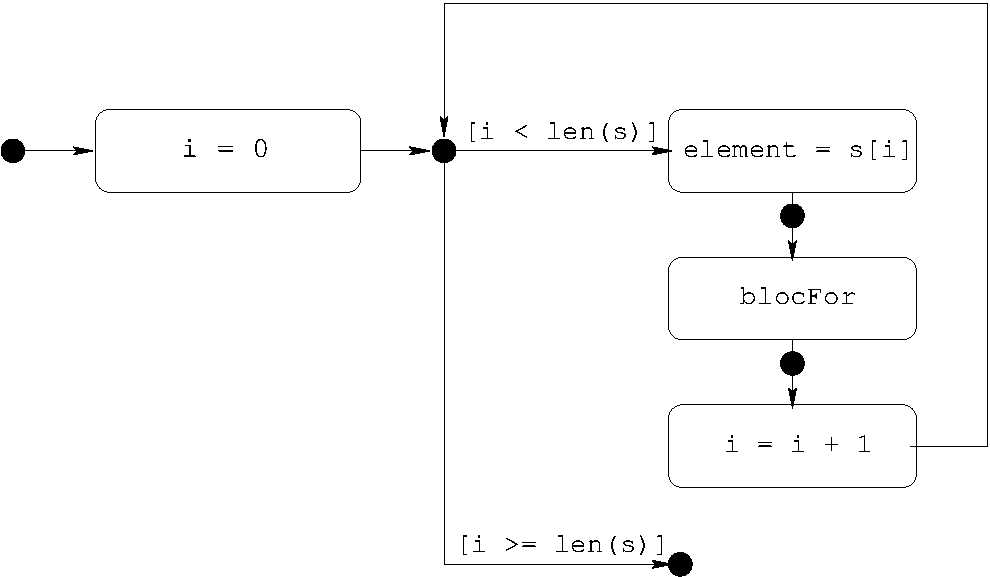
\includegraphics[width=7.5cm]{uml7.pdf}}
\end{fig}

\begin{td}[Suite arithmétique (2)]\label{td:suiteArit2}\index[algo]{suites numériques}
\begin{enumerate}
\item Ecrire un algorithme qui calcule de manière itérative la somme $s = \sum_0^n u_k$ des $n$ premiers 
	termes d'une suite arithmétique $u_k = a + r\cdot k$. On utilisera une boucle {\tt for}.
\item Comparer l'efficacité de cette approche itérative avec le calcul du TD \ref{td:suiteArit} 
	page \pageref{td:suiteArit}.
\end{enumerate}
\end{td}}

\noindent L'affichage précédent nous a conduits à parcourir la chaîne {\tt s}
du premier élément ({\tt i = 0}) au dernier élément ({\tt i = len(s)-1}).
On peut généraliser cet exemple au parcours d'une séquence {\tt s} quelconque, 
du premier élément au dernier élément (parcours direct) :

\index{boucle!parcours de séquence}
\begin{py}{5cm}
\begin{verbatim}
i = 0
while i < len(s):
    # traiter s[i]
    i = i + 1
\end{verbatim}
\end{py}
\hfill
\begin{py}{10cm}
Se placer au début de la séquence : initialiser un entier {\tt i} qui représentera
le rang dans la séquence (rang initial : {\tt i = 0}); puis tant qu'on est dans
la séquence (condition : {\tt 0 <= i < len(s)}), traiter l'élément courant {\tt s[i]} 
et passer à l'élément suivant ({\tt i = i + 1}).
\end{py}\\
\exo{td:parcours}
 
\noindent Il existe une instruction de contrôle adaptée au parcours de séquence (figure \ref{fig:for}) :
\index{for@{{\tt for}}}
$$\fbox{\tt for element in sequence : blocFor}$$
$$\begin{minipage}{6.5cm}équivalente à : 
\begin{py}{4cm}
\begin{verbatim}
i = 0
while i < len(s):
    element = sequence[i]
    blocFor
    i = i + 1
\end{verbatim}
\end{py}
\end{minipage}$$
\noindent Ainsi, l'algorithme de l'exemple \ref{ex:caractere} ci-dessus peur se réécrire 
simplement sous la forme :\\
{\tt \mbox{}\ \ for element in s : print(element)}\\
De même, l'algorithme de calcul de la fonction puissance (exemple \ref{ex:puissance})
peut s'écrire avec une boucle {\tt for} :\\
{\tt
\mbox{}\ \ p = x\\
\mbox{}\ \ for i in range(n) : p = p*x}
\exo{td:suiteArit2}


%-------------------------------------------------------------------------
\subsection{Imbrications de boucles}
%-------------------------------------------------------------------------
De la même manière que l'on peut cascader des alternatives simples
(voir section \ref{sub:alternatives}), on peut encapsuler une boucle 
dans une autre boucle.\index{boucle!boucles imbriquées}

\begin{ex}[Tables de multiplication]\label{ex:tables}\index[algo]{tables de multiplication}
Nous avons affiché une table de multiplication dans l'exemple \ref{ex:table}
page \pageref{ex:table}. Nous voulons maintenant afficher les 9 premières tables de 
multiplication en réutilisant l'algorithme d'affichage d'une seule table. Il nous suffit
pour cela de répéter 9 fois l'algorithme d'affichage d'une table en incrémentant 
le multiplicande $n$ à chaque itération :\\
\mbox{}\ \ \begin{py}{5cm}
\begin{verbatim}
n = 1
while n <= 9:
    i = 1
    while i < 10:
        print(i, '*', n, '=', i*n)
        i = i + 1
    n = n + 1
\end{verbatim}
\end{py}
\hfill
\begin{minipage}[t]{9.5cm}\footnotesize
On initialise {\tt n} à {\tt 1} (on commence par la table de multiplication de $1$),
puis on entre dans la boucle qui fera varier {\tt n} de {\tt 1} à {\tt 9} ({\tt while n <= 9}).
On exécute l'algorithme d'affichage d'une table (exemple \ref{ex:table}) et à la sortie de
cet algorithme, on n'oublie pas d'incrémenter {\tt n} ({\tt n = n + 1}) pour passer à la
table suivante. Et ainsi de suite jusqu'à la table de $9$. Quand $n = 9$, son incrémentation
lui affecte la valeur {\tt 10}, ce qui rend fausse la condition de la boucle ({\tt n <= 9}) :
on sort alors de la boucle extérieure. 
\end{minipage}
\end{ex}
\exo{td:etoile2}

\marginpar{\footnotesize\em\vspace*{-4cm}
\begin{td}[Dessin d'étoiles (2)]\label{td:etoile2}\index[td]{dessin d'étoiles}
Reprendre le TD \ref{td:etoile} page \pageref{td:etoile} en supposant qu'on ne peut 
afficher qu'une étoile à la fois (on s'interdit ici la possibilité d'écrire
{\tt 5*'*'} à la place de {\tt '*****'} par exemple).
\end{td}
\begin{rem}Dans le langage {\sc Pascal}, les blocs d'instructions sont délimités par les 
mots-clés explicites {\tt begin \ldots\ end}. En langage {\sc C}, les blocs d'instructions 
sont délimités par des accolades ({\tt \{ \ldots\ \}}). En {\sc Python}, les blocs sont 
caractérisés par l'indentation identique de chaque instruction du bloc.
\end{rem}

\begin{fig}[Blocs d'instructions]\label{fig:bloc}\mbox{}\\
\centerline{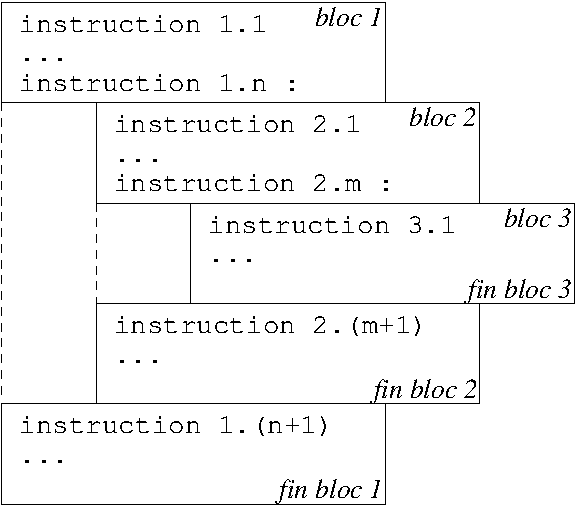
\includegraphics[height=5cm]{bloc.pdf}}
\end{fig}}
\noindent Cet exemple d'instruction composée pose explicitement le problème de la définition
d'un bloc d'instructions : où commence et où termine un bloc d'instructions ?
\index{instruction!bloc d'instructions} 
En effet, l'instruction {\tt n = n + 1} fait-elle partie du bloc de la boucle intérieure
({\tt while i < 10:}) ou du bloc de la boucle extérieure ({\tt while n <= 9:}) ?

Les instructions composées ont toujours la même structure : 
une ligne d'en-tête terminée par un double point ({:}), suivie
d'une ou de plusieurs instructions indentées (décalées à droite)
sous cette ligne d'en-tête (figure \ref{fig:bloc}).

\index{langage!{{\sc Python}}!bloc d'instructions} 
\begin{py}{5cm}
\begin{verbatim}
ligne d'en-tête:
    première instruction du bloc
    ...
    dernière instruction du bloc
    \end{verbatim}
\end{py}

\noindent S'il y a plusieurs instructions indentées sous la ligne d'en-tête, elles doivent l'être exactement au
même niveau (décalage de 4 caractères espace, par exemple). Ces instructions indentées
constituent ce qu'on appellera désormais un bloc d'instructions. Un bloc d'instructions est une
suite d'instructions formant un ensemble logique, qui n'est exécuté que dans certaines conditions
définies dans la ligne d'en-tête. Dans l'exemple précédent, les deux lignes
d'instructions indentées sous la ligne contenant l'instruction « {\tt while i < 10:} » constituent un même 
bloc logique : ces deux lignes ne sont exécutées -- toutes les deux -- que si la condition testée 
avec l'instruction {\tt while} est vérifiée, c'est-à-dire si le multiplicateur {\tt i}
est tel que {\tt 1 <= i < 10}.

\begin{ex}[Tables de vérité]\label{ex:verite}\index[algo]{tables de vérité}
Pour afficher les tables de vérité des opérateurs logiques
de base (voir section \ref{sub:cond}) :
négation (non, {\em not}, $\overline{a}$), 
disjonction (ou, {\em or}, $a+b$) et 
conjonction (et, {\em and}, $a\cdot b$),
on peut utiliser 2 boucles {\tt for} imbriquées :
	
	Exemple : $a\cdot b$ 
	
	\begin{minipage}[t]{5cm}
	$\begin{array}[t]{|c|c|c|}
	\hline
	a & b & a\cdot b\\
	\hline
	0 & 0 & 0\\
	0 & 1 & 0\\
	1 & 0 & 0\\
	1 & 1 & 1\\
	\hline
	\end{array}$
	\end{minipage}
	\hspace*{1cm}
	\begin{py}{5cm}
	\begin{verbatim}
	>>> for a in  [0,1]:
	...   for b in [0,1]:
	...     print(a, b, a and b)
	... 
	0 0 0
	0 1 0
	1 0 0
	1 1 1
	\end{verbatim}
	\end{py}
	\exo{td:booleens2}
\end{ex}


\marginpar{\footnotesize\em\vspace*{-2cm}
\begin{td}[Opérateurs booléens dérivés (2)]\label{td:booleens2}\index[td]{opérateurs booléens dérivés}
A l'aide d'itérations imbriquées, afficher les tables de vérité des 
opérateurs logiques dérivés (voir TD \ref{td:booleens1}) : 
ou exclusif ({\em xor}, $a \oplus b$), 
non ou ({\em nor}, $\overline{a+b}$), 
non et ({\em nand}, $\overline{a\cdot b}$), 
implication ($a \Rightarrow b$) et  
équivalence ($a \Leftrightarrow b$).
\end{td}

\begin{fig}[Nid d'abeilles]\label{fig:abeilles}\mbox{}\\
\centerline{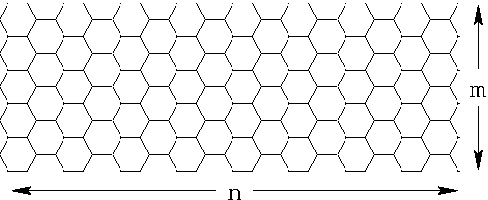
\includegraphics[width=7.5cm]{motif.pdf}}
\end{fig}}
\begin{ex}[Nid d'abeilles]\label{ex:abeille}\index[algo]{nid d'abeilles}\index[td]{nid d'abeilles}
Un motif en nid d'abeilles est
formé de $n\times m$ hexagones en quinconce comme sur la figure \ref{fig:abeilles}
ci-contre.\\
\end{ex}

\noindent Pour dessiner un tel motif, il faut d'abord savoir dessiner un hexagone de côté {\tt a} 
en utilisant les instructions {\em à la {\sc Logo}} de l'annexe \ref{logo} page \pageref{logo} :

\begin{py}{3cm}
\begin{verbatim}
for k in range(6):
    forward(a)
    left(60)
\end{verbatim}
\end{py}
\vspace*{1mm}

\noindent puis une colonne de {\tt m} hexagones de côté {\tt a} à l'abscisse {\tt x0} :

\begin{py}{3cm}
\begin{verbatim}
for j in range(m):
    y0 = a*sqrt(3)*(1/2. - j)
    up()
    goto(-x0,-y0)
    down()
    for k in range(6):
        forward(a)
        left(60)
\end{verbatim}
\end{py}
\vspace*{1mm}

\noindent et enfin {\tt n} colonnes de {\tt m} hexagones en quinconce :

\begin{py}{3cm}
\begin{verbatim}
for i in range(n):
    x0 = -3*i*a/2.
    for j in range(m):
        y0 = a*sqrt(3)*(1/2.*(i%2) - j)
        up()
        goto(-x0,-y0)
        down()
        for k in range(6):
            forward(a)
            left(60)
\end{verbatim}
\end{py}

\marginpar{\footnotesize\em
\begin{td}[Damier]\label{td:damier}\index[td]{damier}
En utilisant les instructions {\em à la {\sc Logo}} de l'annexe \ref{logo} page \pageref{logo},
dessiner un damier rectangulaire de $n\times m$ cases.
\end{td}}

\exo{td:damier}

%-------------------------------------------------------------------------
\subsection{Exécutions de boucles}\label{sub:executionBoucles}
%-------------------------------------------------------------------------
La maîtrise de l'algorithmique requiert deux qualités complémentaires \cite{darmengeat} :
\begin{itemize}
\item il faut avoir une certaine intuition, car aucun algorithme ne permet de 
	savoir {\em a priori} quelles instructions permettront d'obtenir le résultat 
	recherché. C'est là qu'intervient la forme « d'intelligence » 
	requise pour l'algorithmique : la « créativité » de l'informaticien. 
	Il y a des gens qui possèdent au 
	départ davantage cette intuition que les autres.  
	Cependant, les réflexes, cela s'acquiert (en particulier, l'annexe \ref{invariant}
	page \pageref{invariant} présente une méthode pour aider à construire des boucles). 
	Et ce qu'on appelle l'intuition n'est finalement que de l'expérience accumulée,
	tellement répétée que le raisonnement, au départ laborieux, finit par 
	devenir «~spontané~».
\marginpar{\footnotesize\em
\begin{rem}
Si en littérature « lire, c'est écrire dans sa tête », en algorithmique
« lire un algorithme, c'est l'exécuter dans sa tête ». 
\end{rem}}
\item il faut être méthodique et rigoureux. En effet, chaque fois qu'on écrit 
	une série d'instructions que l'on croit justes, il faut systématiquement 
	se mettre mentalement à la place de la machine qui va les exécuter
	(sur papier ou dans sa tête) afin de vérifier si le résultat obtenu 
	est bien celui que l'on voulait. 
	Cette opération ne requiert pas d'intuition. Mais elle reste néanmoins indispensable
	si l'on ne veut pas écrire des algorithmes à l'« aveuglette ».
	Et petit à petit, à force de pratique, on fera
	de plus en plus souvent l'économie de cette dernière étape : 
	l'expérience fera qu'on « verra » le résultat produit par les instructions, 
	au fur et à mesure qu'on les écrira. 
	Naturellement, cet apprentissage est long, et demande des heures de 
	travail patient. 
	Aussi, dans un premier temps, il faut éviter de sauter les étapes : la vérification méthodique, 
	pas à pas, de chacun des algorithmes représente plus de la moitié du travail à accomplir\ldots
	et le gage de progrès.
\end{itemize}

Pour améliorer la compréhension d'une boucle, on peut « tracer » son exécution de tête,
à la main ou par programme. Dans tous les cas, l'idée est de suivre pas à pas
l'évolution des variables qui interviennent dans la boucle : on détermine leur valeur 
juste avant la boucle, à la fin de chaque itération et juste après la boucle.
C'est ce qui a été fait dans l'exemple \ref{ex:pgcd3} page \pageref{ex:pgcd3} du calcul
du pgcd ou on a « pisté » les 3 variables concernées par ce calcul.
\exo{td:traceFactorielle}   

\marginpar{\footnotesize\em
\begin{td}[Trace de la fonction factorielle]\label{td:traceFactorielle}\index[td]{fonction factorielle}
Tracer la fonction factorielle du TD \ref{td:factorielle} page
\pageref{td:factorielle}.
\end{td}}
\begin{ex}[Exécution d'une boucle]\label{ex:execBoucle}
L'exécution pas à pas de l'algorithme ci-dessous donne le tableau
de droite.

\begin{py}{4cm}
\begin{verbatim}
x = 2
n = 4
k = 1
p = x
while k < n:
    p = p*x
    k = k + 1
\end{verbatim}
\end{py}
\hfill
\begin{py}{10cm}
Les variables concernées par la boucle sont essentiellement {\tt k} et {\tt p} 
({\tt n} et {\tt x} ne varient pas  au cours de l'algorithme) :
$$\begin{tabular}{|l|c|c|}
\cline{2-3}
\multicolumn{1}{c|}{} & \tt k & \tt p \\
\hline
avant & 1 & 2 \\
\hline
pendant & 2 & 4 \\
pendant & 3 & 8 \\
pendant & 4 & 16\\
\hline
après & 4 & 16\\
\hline
\end{tabular}$$
\end{py}\\
\end{ex}

\begin{ex}[Nombres de Fibonacci]\label{ex:fibonacci}\index[algo]{nombres de {{\sc Fibonacci}}}
Les nombres de Fibonacci sont donnés par la suite
$\displaystyle \left\{\begin{array}{l}
f_0 = f_1 = 1\\
f_n = f_{n-1} + f_{n-2}\ \forall n > 1
\end{array}\right.$ \\
Les 10 premiers nombres de la suite de Fibonacci valent donc
successivement $f_0 = 1$, $f_1 = 1$, $f_2 = 2$, $f_3 = 3$, 
$f_4 = 5$, $f_5 = 8$, $f_6 = 13$, $f_7 = 21$, $f_8 = 34$, et $f_9 = 55$.
\end{ex}
\noindent Le nombre $f_n$ ($n > 1$) de Fibonacci se calcule selon l'algorithme itératif
suivant :

\begin{py}{4cm}
\begin{verbatim}
f, f1, f2 = 2,1,1
for i in range(3,n+1) :
    f2 = f1
    f1 = f
    f = f1 + f2
\end{verbatim}
\end{py}
\hfill
\begin{py}{10cm}
On trace les 4 variables {\tt i}, {\tt f2}, {\tt f1} et {\tt f}
concernées par la boucle  dans le cas $n = 9$ :
$$\begin{tabular}{|l|c|c|c|c|}
\cline{2-5}
\multicolumn{1}{c|}{} & \tt i & \tt f2 & \tt f1 & \tt f \\
\hline
avant & ? & 1 & 1 & 2 \\
\hline
pendant & 3  & 1  & 2  & 3 \\
pendant & 4  & 2  & 3  & 5 \\
pendant & 5  & 3  & 5  & 8 \\
pendant & 6  & 5  & 8  & 13 \\
pendant & 7  & 8  & 13  & 21 \\
pendant & 8  & 13  & 21  & 34 \\
pendant & 9  & 21  & 34  & 55 \\
\hline
après & 9  & 21  & 34  & 55 \\
\hline
\end{tabular}$$
\end{py}\\
\exo{td:quinconce}
\marginpar{\footnotesize\em
\begin{td}[Figure géométrique]\label{td:quinconce}\index[td]{figure géométrique}
Que dessinent les instructions suivan\-tes ?
\vspace*{1mm}

	{\tt \mbox{}\ \ }\begin{minipage}{5cm}\tt
	x0 = 0\\
	y0 = 0\\
	r = 10\\
	n = 5\\
	m = 10\\
	for i in range(n) :\\
	\mbox{}\ \ \ \ up()\\
	\mbox{}\ \ \ \ y = y0 - 2*r*i\\
	\mbox{}\ \ \ \ x = x0 + r*(i\%2)\\
	\mbox{}\ \ \ \ goto(x,y)\\
	\mbox{}\ \ \ \ for j in range(m) :\\
	\mbox{}\ \ \ \ \ \ \ \ down()\\
	\mbox{}\ \ \ \ \ \ \ \ circle(r)\\
	\mbox{}\ \ \ \ \ \ \ \ up()\\
	\mbox{}\ \ \ \ \ \ \ \ x = x + 2*r\\
	\mbox{}\ \ \ \ \ \ \ \ goto(x,y)
	\end{minipage}
\end{td}}

%-------------------------------------------------------------------------
\subsection{Construction d'une boucle}\label{invariant}
%-------------------------------------------------------------------------
Un algorithme est un mécanisme qui fait passer un « système » d'une « situation »
dite initiale (ou précondition) à une « situation » finale (postcondition ou but). 
Le couple (situation initiale, situation finale) est appelé spécification de l'algorithme. 
L'algorithmique vise donc à construire rationnellement des algorithmes à partir de 
leur spécification.

\begin{ex}[Enfoncer un clou]\label{ex:clou}
On dispose d'une planche, d'un marteau et d'un clou (situation initiale)
et on veut que le clou soit enfoncé dans la planche jusqu'à la tête (situation finale).

Le travail à réaliser consiste donc à planter légèrement le clou
à la main de façon qu'il tienne seul, puis à taper sur la tête du clou avec le marteau
tant que la tête ne touche pas la planche. Le nombre de coups nécessaire est {\em a priori}
inconnu.
\end{ex}
\noindent 
Le raisonnement qui permet de passer d'une compréhension intuitive d'un
tel énoncé à l'algorithme n'est pas toujours facile à concevoir d'un coup. 
Dans le cas d'une boucle on pourra systématiser la conception de l'algorithme
autour de 4 étapes (d'après \cite{didier} et \cite{guyomard}):
\begin{enumerate}
\item {\bf Invariant} (ou hypothèse de récurrence) : « Le clou est planté dans la planche ».
\item {\bf Condition d'arrêt} : « La tête touche la planche ».
\item {\bf Progression} : « Frapper un coup de marteau de façon à enfoncer un peu plus le clou ».
\item {\bf Initialisation} : « Planter légèrement le clou à la main ».
\end{enumerate}
Il faut noter que les étapes 1 et 2 définissent des situations
tandis que les étapes 3 et 4 concernent des actions. 
Dans cette section, on notera les situations entre crochets ({\tt []}) pour les distinguer
des actions.
\begin{itemize}
\item La recherche d'un invariant est l'étape clé autour de laquelle s'articule la conception des boucles. 
	La conjonction de l'invariant et de la condition d'arrêt conduit logiquement au but recherché :
	$$\fbox{\begin{minipage}{13cm}\tt
	[« invariant » and « condition d'arrêt »] $\Rightarrow$ [« postcondition »]
	\end{minipage}}$$
	La condition d'arrêt seule n'implique pas le but : un clou posé sur la
	planche la pointe en l'air a bien la tête qui touche la planche, mais il n'est pas
	planté dans la planche.
\item La progression doit :
	\begin{itemize}
	\item conserver l'invariant (pas de coup de marteau qui déplanterait le clou !).
		Plus précisément, la progression est un fragment d'algorithme
		défini par les situations initiale et finale suivantes :\\
		\mbox{}\hspace*{5mm}situation initiale : {\tt [« invariant » and not « condition d'arrêt »]}\\
		\mbox{}\hspace*{5mm}situation finale : {\tt [« invariant »]}\\ 
		Dans l'exemple du clou, étant donnée la précondition {\tt [« le clou est planté dans la
		planche » and « la tête ne touche pas la planche »]}, et la postcondition {\tt [« le
		clou est enfoncé dans la planche »]}, une solution à la progression est {\tt « frap\-per
		un coup de marteau »}. 
		$$\fbox{\begin{minipage}{13cm}\tt
		\mbox{}[« invariant » and not « condition d'arrêt »]\\
		\mbox{}« progression »\\
		\mbox{}[« invariant »]
		\end{minipage}}$$
	\item faire effectivement progresser vers le but pour faire en sorte que la condition 
		d'arrêt soit atteinte au bout d'un temps fini. Ici il est nécessaire de
		faire décroître la hauteur du clou au dessus de la planche. 
	\end{itemize}
\item  L'initialisation doit instaurer l'invariant. 
	Plus précisément, elle doit, partant de la précondi\-tion, atteindre l'invariant.
		$$\fbox{\begin{minipage}{13cm}\tt
		\mbox{}[« précondition »]\\
		\mbox{}« initialisation »\\
		\mbox{}[« invariant »]
		\end{minipage}}$$

\end{itemize}
Pour enfoncer un clou dans une planche, on exécutera ainsi l'algorithme suivant :
$$\begin{minipage}[t]{10cm}
\begin{verbatim}
[« on dispose d'une planche d'un marteau, d'un clou »]
« Planter légèrement le clou à la main »
[« le clou est planté dans la planche »]
while [« la tête du clou ne touche pas la planche »] :
    « frapper un coup de marteau sur la tête du clou »
    [« le clou est planté dans la planche »]
[« le clou est enfoncé dans la planche »]
\end{verbatim}
\end{minipage}$$

D'une manière plus générale, les 4 étapes de construction d'une boucle
sont les suivantes :
\marginpar{\footnotesize\em
\begin{fig}[Invariant de boucle]\label{fig:invariant}\mbox{}\\
\centerline{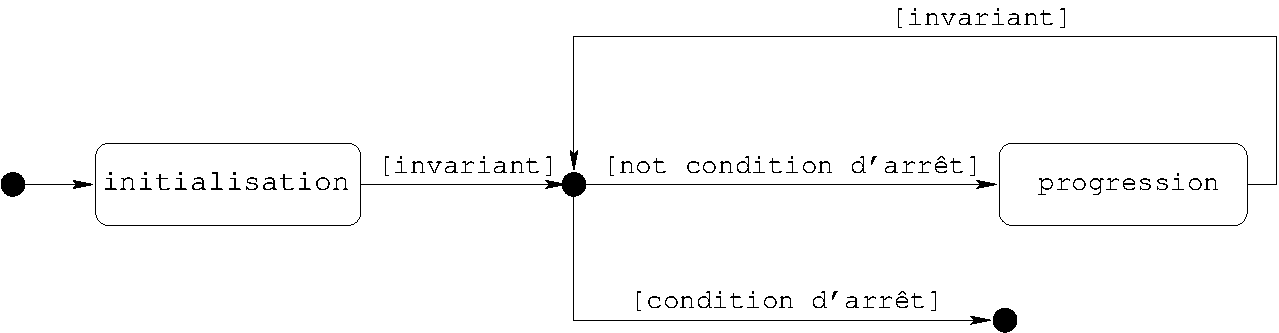
\includegraphics[width=7.5cm]{uml5.pdf}}
\vspace*{3mm}

Dans la pratique, on ne teste pas les invariants.
\vspace*{2mm}

\centerline{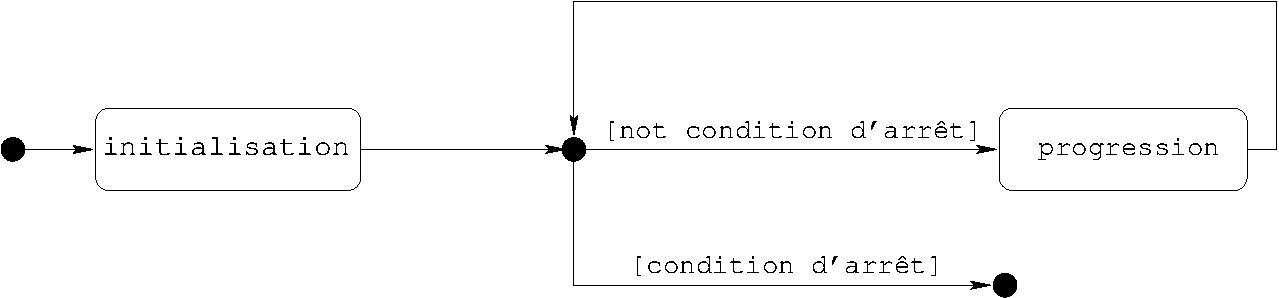
\includegraphics[width=7.5cm]{uml6.pdf}}
\end{fig}}
\begin{enumerate}
\item {\bf Invariant :} proposer une situation générale décrivant le problème posé (hypothèse de
	récurrence). C'est cette étape qui est la plus délicate car elle exige de faire 
	preuve d'imagination.
	
	\begin{minipage}[t]{6cm}
	Exemple de la puissance \ref{ex:puissance} :\\
	$x^{k+1} = x\cdot x^k$
	\end{minipage}
	\hfill
	\begin{minipage}[t]{6cm}
	Exemple du pgcd \ref{ex:pgcd3} :\\
	${\rm pgcd}(a,b) = {\rm pgcd}(b,a \bmod b)$
	\end{minipage}
\item {\bf Condition d'arrêt :} \index{boucle!condition d'arrêt} à partir de la situation générale imaginée en [1], on doit
	formuler la condition qui permet d'affirmer que l'algorithme a terminé son travail. 
	La situation dans laquelle il se trouve alors est appelée situation finale.
	La condition d'arrêt fait sortir de la boucle.
	
	\begin{minipage}[t]{6cm}
	Exemple de la puissance \ref{ex:puissance} :\\
	{\tt k > n}
	\end{minipage}
	\hfill
	\begin{minipage}[t]{6cm}
	Exemple du pgcd \ref{ex:pgcd3} :\\
	{\tt b == 0}
	\end{minipage}
\item {\bf Progression :} se « rapprocher » de la situation finale, tout en faisant le nécessaire pour
	conserver à chaque étape une situation générale analogue à celle retenue en [1].
	La progression conserve l'invariant.
	
	\begin{minipage}[t]{6cm}
	Exemple de la puissance \ref{ex:puissance} :\\
	{\tt p = p*x}\\
	{\tt k = k + 1}
	\end{minipage}
	\hfill
	\begin{minipage}[t]{6cm}
	Exemple du pgcd \ref{ex:pgcd3} :\\
	{\tt r = a\%b}\\
	{\tt a = b}\\
	{\tt b = r}
	\end{minipage}
\item {\bf Initialisation :} initialiser les variables introduites dans l'invariant 
	pour que celui-ci soit vérifié avant d'entrer dans la boucle.
	L'initialisation « instaure » l'invariant.
	
	\begin{minipage}[t]{6cm}
	Exemple de la puissance \ref{ex:puissance} :\\
	{\tt k = 1}\\
	{\tt p = x}
	\end{minipage}
	\hfill
	\begin{minipage}[t]{6cm}
	Exemple du pgcd \ref{ex:pgcd3} :\\
	---
	\end{minipage}
\item {\bf Boucle finale :} Une fois les 4 étapes précédentes menées à leur terme, l'algorithme recherché 
	aura la structure finale suivante (figure \ref{fig:invariant}) :
	$$\begin{minipage}[t]{4cm}
	\begin{verbatim}
	[« précondition »]
	« initialisation »
	[« invariant »]
	while not [« condition d'arrêt »] :
	    « progression »
	    [« invariant »]
	[« postcondition »]
	\end{verbatim}
	\end{minipage}$$
	Quand on sort de la boucle, la situation finale attendue est atteinte.
	
	Dans la pratique, on ne garde que les instructions :
	$$\fbox{\begin{minipage}[t]{8cm}\tt
	« initialisation »\\
	while [not « condition d'arrêt »] : \\
	\mbox{}\ \ \ \ « progression »
	\end{minipage}}$$
	\begin{minipage}[t]{6cm}
	Exemple de la puissance \ref{ex:puissance} :\\
	{\tt k = 1}\\
	{\tt p = x}\\
	{\tt while not k > n: }\\
	{\tt \mbox{}\ \ \ \ p = p*x}\\
	{\tt \mbox{}\ \ \ \ k = k + 1}
	\end{minipage}
	\hfill
	\begin{minipage}[t]{6cm}
	Exemple du pgcd \ref{ex:pgcd3} :\\
	{\tt while not b == 0:}\\
	{\tt \mbox{}\ \ \ \ r = a\%b}\\
	{\tt \mbox{}\ \ \ \ a = b}\\
	{\tt \mbox{}\ \ \ \ b = r}
	\end{minipage}
	\vspace*{2mm}
	
	Un des problèmes, pour l'apprenti informaticien, est que la boucle finale
	ainsi obtenue ne fait pas apparaître explicitement l'invariant dans le code. 
	L'invariant est une aide conceptuelle pour construire la boucle, 
	mais pas pour l'exécuter.
\end{enumerate}
\exo{td:suiteArit3}
\marginpar{\footnotesize\em\vspace*{-5cm}
\begin{rem}
Cette façon de procéder permet de « prouver » la validité de l'algorithme au fur et à
mesure de son élaboration. En effet la situation générale choisie en [1] est en fait l'invariant 
qui caractérise la boucle {\tt while}.
Cette situation est satisfaite au départ grâce à l'initialisation de l'étape [4]; 
elle reste vraie à chaque itération (étape [3]). Ainsi lorsque la condition d'arrêt (étape [2])
est atteinte cette situation nous permet d'affirmer que le problème est résolu.
C'est également en analysant l'étape [3] qu'on peut prouver la terminaison de l'algorithme.
\end{rem}

\begin{td}[Suite arithmétique (3)]\label{td:suiteArit3}
Reprendre le TD \ref{td:suiteArit2} page \pageref{td:suiteArit2} en explicitant l'invariant, la condition d'arrêt,
la progression et l'initialisation de la boucle retenue.
\end{td}}

\begin{defin}[invariant de boucle]\index[def]{invariant de boucle}\index{boucle!invariant}
Un invariant de boucle est une propriété vérifiée tout au long de 
l'exécution de la boucle. 
\end{defin}

	
%-------------------------------------------------------------------------
\newpage
\setlength{\textwidth}{25cm}
\setlength{\textheight}{16cm}
\setlength{\marginparwidth}{0cm}
\setlength{\marginparsep}{0cm}
\setlength{\linewidth}{25cm}
\setlength{\oddsidemargin}{0cm}
\setlength{\evensidemargin}{0cm}
\setlength{\topmargin}{-0.75cm}

\section{Exercices complémentaires}
%-------------------------------------------------------------------------

%-------------------------------------------------------------------------
\subsection{Connaître}
%-------------------------------------------------------------------------
\begin{td}[QCM (2)]\label{td:qcmInstruc}\index{evaluation@évaluation!contrôle d'attention}\index[td]{contrôle d'attention}(un seul item correct par question)
\em
\begin{enumerate}
\item En {\sc Python}, l'instruction « ne rien faire » se dit
	\begin{enumerate}
	\item {\tt break}
	\item {\tt return}
	\item {\tt pass}
	\item {\tt continue}
	\end{enumerate}
\item Une variable informatique est un objet 
	\begin{enumerate}
	\item équivalent à une variable mathématique
	\item qui associe un nom à une valeur
	\item qui varie nécessairement
	\item qui modifie la mémoire
	\end{enumerate}
\item L'affectation consiste à
	\begin{enumerate}
	\item comparer la valeur d'une variable à une autre valeur
	\item associer une valeur à une variable
	\item incrémenter une variable
	\item déplacer une variable en mémoire
	\end{enumerate}
\item Après la séquence \fbox{\footnotesize\tt\begin{tabular}{l}a = 13\\b = 4\\b = a\\a = b\end{tabular}} les variables {\tt a} et {\tt b} sont telles que
	\begin{enumerate}
	\item {\tt a = 13} et {\tt b = 13}
	\item {\tt a = 4} et {\tt b = 4}
	\item {\tt a = 4} et {\tt b = 13}
	\item {\tt a = 13} et {\tt b = 4}
	\end{enumerate}
\item Le résultat d'une comparaison est une valeur
	\begin{enumerate}
	\item réelle
	\item qui dépend du type des arguments 
	\item booléenne
	\item entière
	\end{enumerate}
\item Un opérateur booléen s'applique à des valeurs
	\begin{enumerate}
	\item booléennes
	\item entières
	\item réelles
	\item alphanumériques
	\end{enumerate}
\item La fonction principale d'une instruction de test est
	\begin{enumerate}
	\item de passer d'instruction en instruction
	\item de répéter une instruction sous condition
	\item d'exécuter une instruction sous condition
	\item d'interrompre l'exécution d'une instruction
	\end{enumerate}
\item Après la séquence \fbox{\footnotesize\tt\begin{tabular}{l}x = -3\\if   x < -4 : y = 0\\elif x < -3 : y = 4 - x\\elif x < -1 : y = x*x + 6*x + 8\\elif x < 3 : y = 2 - x\\else : y = -2\end{tabular}} la variable {\tt y} est telle que
	\begin{enumerate}
	\item {\tt y = -1}
	\item {\tt y = 0}
	\item {\tt y = 7}
	\item {\tt y = -2}
	\end{enumerate}
\item L'itération conditionnelle est une instruction de contrôle du flux d'instructions 
	\begin{enumerate}
	\item qui permet d'exécuter une instruction sous condition préalable.
	\item qui est vérifiée tout au long de son exécution. 
	\item qui permet sous condition préalable de répéter zéro ou plusieurs fois la même instruction.
	\item qui permet de choisir entre plusieurs instructions.
	\end{enumerate}
\item On ne sort jamais d'une boucle si la condition d'arrêt 
	\begin{enumerate}
	\item ne varie pas en cours d'exécution.
	\item ne contient pas d'opérateurs booléens.
	\item est toujours fausse.
	\item n'est jamais fausse.
	\end{enumerate}
\item Que vaut {\tt f} à la fin des instructions suivantes si $n = 5$ ?

	\begin{py}{4cm}
	\begin{verbatim}
	f = 0
	i = 1
	while i < n+1:
	    f = f + i
	    i = i + 1
	\end{verbatim}
	\end{py}

	\begin{enumerate}
	\item 6
	\item 10
	\item 15
	\item 21
	\end{enumerate}
\item Une séquence est une suite ordonnée 
	\begin{enumerate}
	\item d'éléments que l'on peut référencer par leur rang.
	\item d'instructions formant un ensemble logique.
	\item d'instructions conditionnelles.
	\item de nombres
	\end{enumerate}
\item Dans la chaîne {\tt s = 'gérard'}, {\tt s[2]} vaut
	\begin{enumerate}
	\item {\tt 'é'}
	\item {\tt 'r'}
	\item {\tt 'gé'}
	\item {\tt 'gér'}
	\end{enumerate}
\item Que vaut {\tt f} à la fin des instructions suivantes si $n = 5$ ?

	\begin{py}{4cm}
	\begin{verbatim}
	f = 1
	for i in range(2,n+1) :
	    f = f * i
	\end{verbatim}
	\end{py}

	\begin{enumerate}
	\item 120
	\item 720
	\item 6
	\item 24
	\end{enumerate}
\item Que vaut {\tt f} à la fin des instructions suivantes si $n = 5$ ?

	\begin{py}{4cm}
	\begin{verbatim}
	f, f1, f2 = 2,1,1
	for i in range(3,n+1) :
	    f2 = f1
	    f1 = f
	    f = f1 + f2
	\end{verbatim}
	\end{py}

	\begin{enumerate}
	\item 3
	\item 5
	\item 8
	\item 13
	\end{enumerate}
\end{enumerate}
\end{td}


%-------------------------------------------------------------------------
\subsection{Comprendre}
%-------------------------------------------------------------------------
\begin{td}[Unité de longueur]\label{td:al}\em \index[td]{unité de longueur}
L'année-lumière (al) est une unité de distance utilisée en astronomie. 
Une année-lumière est la distance parcourue par un photon (ou plus simplement la lumière) 
dans le vide, en dehors de tout champ gravitationnel ou magnétique, en une année julienne 
(365,25 jours). 

Ecrire une instruction qui permette de passer directement des années-lumière aux m/s sachant que
la vitesse de la lumière dans le vide est de 299 792 458 m/s.
\end{td}

\begin{td}[Permutation circulaire (2)]\label{td:permutation2}\em \index[algo]{permutation circulaire}\index[td]{permutation circulaire}
 Effectuer une permutation circulaire gauche entre les valeurs de 3 entiers $x$, $y$ et $z$.
\end{td}

\begin{td}[Séquence d'affectations (2)]\label{td:seq2}\em \index[td]{séquence d'affectations}
	Quelles sont les valeurs des variables $n$ et $s$
	après la séquence d'affectations suivante ?
	
	\noindent{\footnotesize\tt
	\mbox{}\ \ n = 1\\
	\mbox{}\ \ s = n\\
	\mbox{}\ \ n = n + 1\\
	\mbox{}\ \ s = s + n\\
	\mbox{}\ \ n = n + 1\\
	\mbox{}\ \ s = s + n\\
	\mbox{}\ \ n = n + 1\\
	\mbox{}\ \ s = s + n\\
	\mbox{}\ \ n = n + 1\\
	\mbox{}\ \ s = s + n
	}
\end{td}

\begin{td}[Circuits logiques (2)]\label{td:circuits2}\em \index[algo]{circuits logiques}\index[td]{circuits logiques}
On considère les conventions graphiques traditionnelles pour les opérateurs logiques :
$$\begin{tabular}{ccccccc}
$\overline{a}$ & $a \cdot b$ & $a + b$ & $a \oplus b$ & $a \cdot b \cdot c$ & $a + b + c$ & $\overline{a \cdot b \cdot c}$ \\
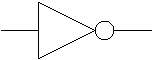
\includegraphics[height=1cm]{non.pdf} & 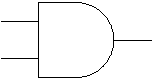
\includegraphics[height=1cm]{et.pdf} & 
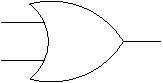
\includegraphics[height=1cm]{ou.pdf}  & 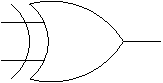
\includegraphics[height=1cm]{xor.pdf} & 
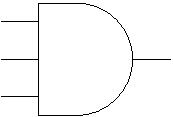
\includegraphics[height=1cm]{et3.pdf} & 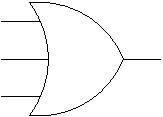
\includegraphics[height=1cm]{ou3.pdf} & 
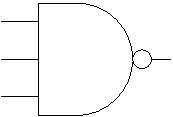
\includegraphics[height=1cm]{nonet3.pdf}
\end{tabular}$$
Donner les séquences d'affectations permettant de calculer la (ou les) sortie(s)
des circuits logiques suivants en fonction de leurs entrées.

\begin{minipage}[t]{8cm}
\begin{enumerate}
\item $a$ et $b$ sont les entrées, $s$ la sortie.
	$$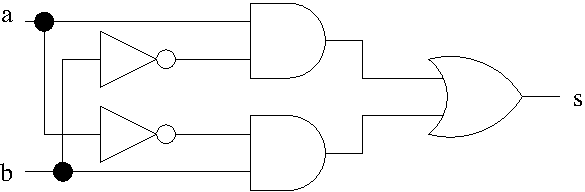
\includegraphics[width=6cm]{ex1.pdf}$$
\end{enumerate}
\end{minipage}
\hfill
\begin{minipage}[t]{8cm}
\begin{enumerate}\setcounter{enumi}{1}
\item $a$ et $b$ sont les entrées, $s$ la sortie.
	$$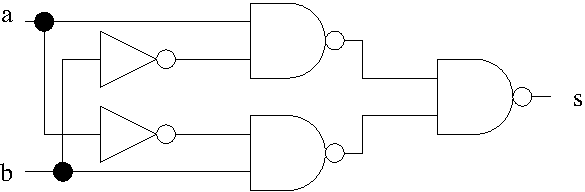
\includegraphics[width=6cm]{ex2.pdf}$$
\end{enumerate}
\end{minipage}

\begin{minipage}[t]{8cm}
\begin{enumerate}\setcounter{enumi}{2}
\item $a$ et $b$ sont les entrées, $s$ et $t$ les sorties.	
	$$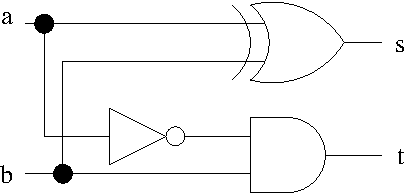
\includegraphics[width=4.5cm]{demiSous.pdf}$$
\item $a$, $b$ et $c$ sont les entrées, $s$ et $t$ les sorties.
	$$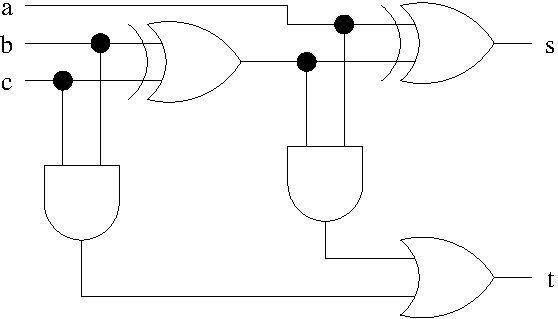
\includegraphics[width=5cm]{add3.pdf}$$
\item $a$, $b$ et $c$ sont les entrées et $s$ la sortie.
	$$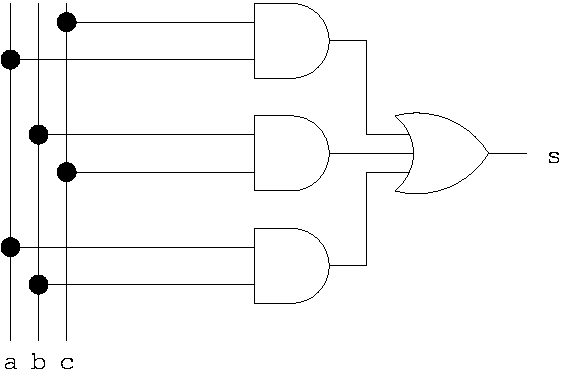
\includegraphics[width=5cm]{majorite.pdf}$$
\end{enumerate}
\end{minipage}
\hfill
\begin{minipage}[t]{8cm}
\begin{enumerate}\setcounter{enumi}{5}
\item $a$, $b$ et $c$ sont les entrées, $s$ et $t$ les sorties.
	$$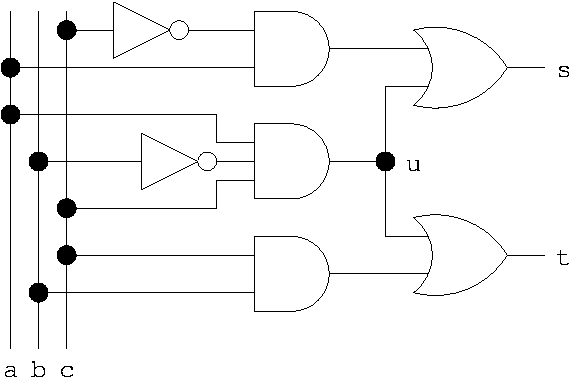
\includegraphics[width=5cm]{circuit.pdf}$$
\item $a$, $b$ et $c$ sont les entrées, $s$ la sortie.
	$$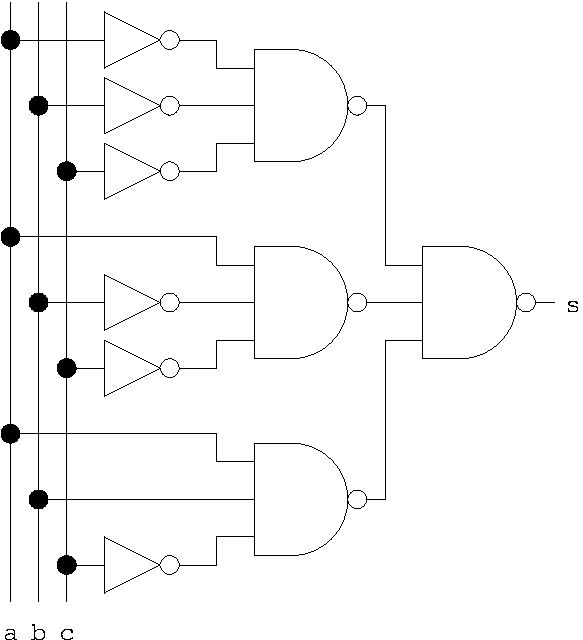
\includegraphics[width=5cm]{f3.pdf}$$
\end{enumerate}
\end{minipage}

\begin{minipage}[t]{8cm}
\begin{enumerate}\setcounter{enumi}{7}
\item $a$, $b$ et $c$ sont les entrées, $s_0$,$s_1$\ldots $s_7$ les sorties.
	$$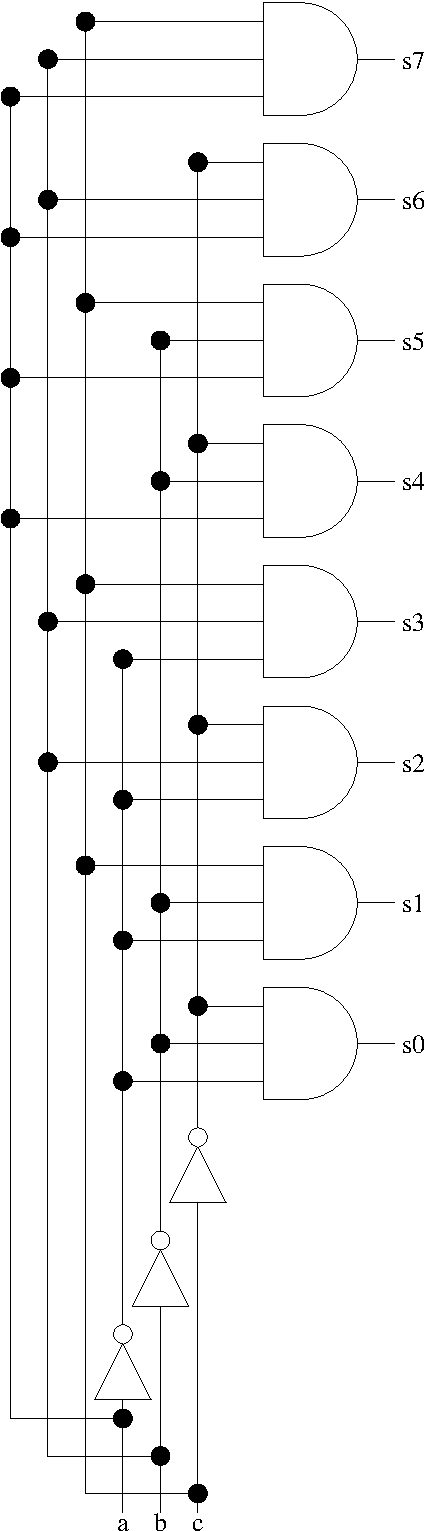
\includegraphics[width=4cm]{decodeur.pdf}$$
\end{enumerate}
\end{minipage}
\end{td}

\begin{td}[Alternative simple et test simple]\label{td:reciproque}\em \index[td]{alternative simple et test simple}
Montrer à l'aide d'un contre-exemple que l'alternative simple
de la figure \ref{fig:alternative} page \pageref{fig:alternative}
n'est pas équivalente à la séquence de tests simples suivante :\\
{\tt
\mbox{}\ \ if condition : blocIf\\
\mbox{}\ \ if not condition : blocElse
}
\end{td}

\begin{td}[Racines du trinome]\label{td:trinome}\em \index[algo]{racines du trinome}\index[td]{racines du trinome}
Ecrire un algorithme qui calcule les racines $x_1$ et $x_2$ du trinome $ax^2 + bx + c$.
\end{td}

\begin{td}[Séquences de tests]\label{td:seq3}\em \index[td]{séquences de tests}
\begin{enumerate}
\item Quelle est la valeur de la variable $x$ après la suite
	d'instructions suivante ?

	{\footnotesize\tt
	x = -3\\
	if x < 0 : x = -x
	}
\item Quelle est la valeur de la variable $y$ après la suite
	d'instructions suivante ?

	{\footnotesize\tt
	x0 = 3\\
	x = 5\\
	if x < x0 : y = -1\\
	else : y = 1
	}
\item Quelle est la valeur de la variable $y$ après la suite
	d'instructions suivante ?

	{\footnotesize\tt
	p = 1\\
	d = 0\\
	r = 0\\
	h = 1\\
	z = 0\\
	f = p and (d or r)\\
	g = not r \\
	m = not p and not z\\
	g = g and (d or h or m)\\
	if f or g : y = 1\\
	else : y = 0
	}
\item Quelle est la valeur de la variable $ok$ après la suite
	d'instructions suivante ?

	{\footnotesize\tt
	x = 2\\
	y = 3\\
	d = 5\\
	h = 4\\
	if x > 0 and x < d :\\
  	\mbox{}\ \ if y > 0 and y < h : ok = 1\\
	\mbox{}\ \ else : ok = 0\\
	else : ok = 0
	}
\item Quelle est la valeur de la variable $y$ après la suite
	d'instructions suivante ?

	{\footnotesize\tt
	x = 3\\
	y = -2\\
	if x < y : y = y - x\\
	elif x == y : y = 0\\
	else : y = x - y
	}
\end{enumerate}
\end{td}
 
\begin{td}[Racine carrée entière]\label{td:racine}\em \index[algo]{racine carrée entière}\index[td]{racine carrée entière}
Ecrire un algorithme qui calcule la racine carrée entière $r$ 
d'un nombre entier positif $n$ telle que $r^2 \leq n < (r+1)^2$.
\end{td}

\begin{td}[Exécutions d'instructions itératives]\label{td:iterations}\em \index[td]{exécutions d'instructions itératives}
\begin{minipage}[t]{8cm}
\begin{enumerate}
\item Que fait cette suite d'instructions ?

	{\footnotesize\tt
	x = 0\\
	while x != 33 :\\
	\mbox{}\ \ x = input('entrer un nombre : ')
	}
\item Que fait cette suite d'instructions ?

	{\footnotesize\tt
	x = 0\\
	while x <= 0 or x > 5 :\\
	\mbox{}\ \ x = input('entrer un nombre : ')
	}
\item Que fait cette suite d'instructions ?

	{\footnotesize\tt
	s = 0\\
	for i in range(5) :\\
	\mbox{}\ \ x = input('entrer un nombre : ')\\
	\mbox{}\ \ s = s + x
	}
\end{enumerate}
\end{minipage}
\hfill
\begin{minipage}[t]{8cm}
\begin{enumerate}\setcounter{enumi}{3}
\item Qu'affichent les itérations suivantes ?

	{\footnotesize\tt
	for i in range(0,10) :\\
	\mbox{}\ \ for j in range(0,i) :\\
	\mbox{}\ \ \ \ print('*',end=' ')\\
	\mbox{}\ \ print()
	}
\item Qu'affichent les itérations suivantes ?

	{\footnotesize\tt
	for i in range(0,10) :\\
	\mbox{}\ \ j = 10 - i\\
	\mbox{}\ \ while j > 0 :\\
	\mbox{}\ \ \ \ print('*',end=' ')\\
	\mbox{}\ \ \ \ j = j - 1\\
	\mbox{}\ \ print()
	}
\end{enumerate}
\end{minipage}

\begin{minipage}[t]{8cm}
\begin{enumerate}\setcounter{enumi}{5}
\item Qu'affichent les itérations suivantes ?

	{\footnotesize\tt
	for i in range(1,10):\\
	\mbox{}\ \ for j in range(0,11) :\\
	\mbox{}\ \ \ \ print(i, 'x', j, ' = ', i*j)\\
	\mbox{}\ \ print()
	}
\item Qu'affichent les itérations suivantes ?\index[algo]{coefficients du binôme}

	{\footnotesize\tt
	for n in range(10) :\\
  	\mbox{}\ \ for p in range(n+1) :\\
    	\mbox{}\ \ \ \ num = 1\\
    	\mbox{}\ \ \ \ den = 1\\
    	\mbox{}\ \ \ \ for i in range(1,p+1) :\\
      	\mbox{}\ \ \ \ \ \ num = num*(n-i+1)\\
      	\mbox{}\ \ \ \ \ \ den = den*i\\
    	\mbox{}\ \ \ \ c = num/den\\
    	\mbox{}\ \ \ \ print(c,end=' ')\\
  	\mbox{}\ \ print()
	}
\end{enumerate}
\end{minipage}
\hfill
\begin{minipage}[t]{8cm}
\begin{enumerate}\setcounter{enumi}{7}
\item Qu'affichent les itérations suivantes ?\index[algo]{nombres de {{\sc Fibonacci}}}

	{\footnotesize\tt
	for n in range(0,15) :\\
  	\mbox{}\ \ f = 1\\
  	\mbox{}\ \ f1 = 1\\
  	\mbox{}\ \ f2 = 1\\
  	\mbox{}\ \ for i in range(2,n+1) :\\
    	\mbox{}\ \ \ \ f = f1 + f2\\
    	\mbox{}\ \ \ \ f2 = f1\\
    	\mbox{}\ \ \ \ f1 = f\\
  	\mbox{}\ \ print(f,end=' ')
	}
\item Quelle est la valeur de la variable $s$
	à la fin des instructions suivantes ?\index[algo]{codage en base $b$}

	{\footnotesize\tt
	b = 2\\
	k = 8\\
	n = 23\\
	s = 0\\
	i = k - 1\\
	q = n\\
	while q != 0 and i >= 0 :\\
  	\mbox{}\ \ s = s + (q\%b)*b**(k-1-i)\\
  	\mbox{}\ \ print(q\%b,end=' ')\\
  	\mbox{}\ \ q = q/b\\
  	\mbox{}\ \ i = i - 1
	}
\end{enumerate}
\end{minipage}
\end{td}


%-------------------------------------------------------------------------
\subsection{Appliquer}
%-------------------------------------------------------------------------
\begin{td}[Figures géométriques]\label{td:geometrieInstruc}\em \index[td]{figure géométrique}
\begin{enumerate}
\item Ecrire un algorithme qui calcule le périmètre $p$ et la surface $s$ d'un rectangle de longueur
	$L$ et de largeur $l$.
\item Ecrire un algorithme qui calcule le périmètre $p$ et la surface $s$ d'un cercle de rayon $r$.
\item Ecrire un algorithme qui calcule la surface latérale $s$ et le volume $v$ d'un cylindre de rayon $r$
	et de hauteur $h$.
\item Ecrire un algorithme qui calcule la surface $s$ et le volume $v$ d'une sphère de rayon $r$.
\end{enumerate}
\end{td}

\begin{td}[Suites numériques]\label{td:suites}\em \index[algo]{suites numériques}\index[td]{suites numériques}
\begin{enumerate}
\item Ecrire un algorithme qui calcule la somme $s = \sum_0^n u_k$ des $n$ premiers termes d'une suite 
	arithmétique $u_k = a + bk$.
\item Ecrire un algorithme qui calcule la somme $s = \sum_0^n u_k$ des $n$ premiers termes d'une suite 
	géométrique $u_k = ab^k$.
\end{enumerate}
\end{td}

\begin{td}[Calcul vectoriel]\label{td:vecteurs}\em \index[algo]{calcul vectoriel}\index[td]{calcul vectoriel}
\begin{enumerate}
\item Ecrire un algorithme qui calcule le module $r$ et les cosinus directeurs $a$, $b$ et $c$
	d'un vecteur de composantes $(x,y,z)$.
\item Ecrire un algorithme qui calcule le produit scalaire $p$ de 2 vecteurs de composantes
	respectives $(x_1,y_1,z_1)$ et $(x_2,y_2,z_2)$.
\item Ecrire un algorithme qui calcule les composantes $(x_3,y_3,z_3)$ du produit vectoriel
	de 2 vecteurs de composantes respectives $(x_1,y_1,z_1)$ et $(x_2,y_2,z_2)$.
\item Ecrire un algorithme qui calcule le produit mixte $v$ de 3 vecteurs de composantes
	respectives $(x_1,y_1,z_1)$, $(x_2,y_2,z_2)$ et $(x_3,y_3,z_3)$.
\end{enumerate}
\end{td}

\begin{td}[Prix d'une photocopie]\label{td:photocopie}\em \index[td]{prix d'une photocopie}
Ecrire un algorithme qui affiche le prix de $n$ photocopies sachant que
	le reprographe facture 0,10 E les dix premières photocopies, 0,09 E 
	les vingt suivantes et 0,08 E au-delà.
\end{td} 

\begin{td}[Calcul des impôts]\label{td:impot}\em \index[td]{calcul des impôts}
Ecrire un algorithme qui affiche si un contribuable d'un pays imaginaire
	est imposable ou non sachant que :
	\begin{itemize}
	\item les hommes de plus de 18 ans paient l'impôt,
    	\item les femmes paient l'impôt si elles ont entre 18 et 35 ans,
	\item les autres ne paient pas d'impôt.
	\end{itemize}
\end{td}


\begin{td}[Développements limités]\label{td:dev}\em \index[algo]{développements limités}\index[td]{développements limités}
Calculer chaque fonction ci-dessous en fonction de son d\'eveloppement 
en série entière ($\sum u_k$). Les calculs seront arr\^et\'es lorsque la 
valeur absolue du terme $u_k$ sera inf\'erieure \`a un certain seuil $s$ 
($0 < s < 1$).\\
On n'utilisera ni la fonction {\em puissance} ($x^n$) ni la fonction 
{\em facto\-riel\-le} ($n!$).
\begin{enumerate}
\item $\displaystyle\sinh(x) \approx \sum_{k=0}^{n} \frac{x^{2k+1}}{(2k+1)!} = 
	x + \frac{x^3}{6} + \frac{x^5}{120} + \ldots + \frac{x^{2n+1}}{(2n+1)!}$
\item $\displaystyle\cosh(x) \approx \sum_{k=0}^{n} \frac{x^{2k}}{(2k)!} = 
	1 + \frac{x^2}{2} + \frac{x^4}{24} + \ldots + \frac{x^{2n}}{(2n)!}$
\item $\displaystyle\cos(x) \approx \sum_{k=0}^{n} (-1)^k\frac{x^{2k}}{(2k)!} = 
	1 - \frac{x^2}{2} + \frac{x^4}{24} + \ldots + (-1)^n\frac{x^{2n}}{(2n)!}$
\item $\displaystyle\log(1+x) \approx \sum_{k=0}^{n} (-1)^k\frac{x^{k+1}}{k+1} = 
	x - \frac{x^2}{2} + \frac{x^3}{3} + \ldots + (-1)^n\frac{x^{n+1}}{n+1}$\ , 
	pour $-1 < x < 1$
\item $\displaystyle\arctan(x) \approx \sum_{k=0}^{n} (-1)^k \frac{x^{2k+1}}{(2k+1)} = 
	x - \frac{x^3}{3} + \frac{x^5}{5} + \ldots + (-1)^n \frac{x^{2n+1}}{(2n+1)}$\ , 
	pour $-1 < x < 1$
\end{enumerate}
\end{td}

\begin{td}[Tables de vérité]\label{td:tablesVerite}\em \index[td]{tables de vérité}
A l'aide d'itérations imbriquées, afficher les tables de vérité des circuits
	logiques du TD \ref{td:circuits2} page \pageref{td:circuits2}.
\end{td}

%-------------------------------------------------------------------------
\subsection{Analyser}
%-------------------------------------------------------------------------
\begin{td}[Dessins géométriques]\label{td:dessins}\em \index[td]{dessins géométriques}
\begin{minipage}[t]{7cm}
	\begin{enumerate}
	\item Que dessine la suite d'instructions suivante ?

		{\footnotesize\tt
		forward(20)\\
		right(144)\\
		forward(20)\\
		right(144)\\
		forward(20)\\
		right(144)\\
		forward(20)\\
		right(144)\\
		forward(20)\\
		right(144)
		}
	\end{enumerate}
\end{minipage}
\hfill
\begin{minipage}[t]{7cm}
	\begin{enumerate}\setcounter{enumi}{1}
	\item Que dessine la suite d'instructions suivante ?

		{\footnotesize\tt 
		forward(10)\\
		left(45)\\
		forward(10)\\
		left(135)\\
		forward(10)\\
		left(45)\\
		forward(10)\\
		left(135)
		}
	\end{enumerate}
\end{minipage}
\end{td}

\begin{td}[Police d'assurance]\label{td:assurance}\em \index[td]{police d'assurance}
Une compagnie d'assurance automobile propose 4 familles de tarifs du moins
	cher au plus onéreux : A, B, C et D. 
	Le tarif dépend de la situation du conducteur.
	\begin{itemize}
	\item Un conducteur de moins de 25 ans et titulaire du permis depuis 
		moins de deux ans, se voit attribuer le tarif D 
		s'il n'a jamais été responsable d'accident. 
		Sinon, la compagnie refuse de l'assurer.
	\item Un conducteur de moins de 25 ans et titulaire du permis depuis plus de deux ans, 
		ou de plus de 25 ans mais titulaire du permis depuis moins de deux ans 
		a le droit au tarif C s'il n'a jamais provoqué d'accident, 
		au tarif D pour un accident, sinon il est refusé.
	\item Un conducteur de plus de 25 ans titulaire du permis depuis plus de deux ans 
		bénéficie du tarif B s'il n'est à l'origine d'aucun accident 
		et du tarif C pour un accident, du tarif D pour deux accidents, 
		et refusé sinon.
	\end{itemize}
	Par ailleurs, pour encourager la fidélité de ses clients, 
	la compagnie propose un contrat au tarif immédiatement inférieur 
	s'il est assuré depuis plus d'un an.
	
	Ecrire un algorithme qui propose un tarif d'assurance selon les caractéristiques
	d'un client potentiel.
\end{td}


\begin{td}[Zéro d'une fonction]\label{td:zero}\em \index[algo]{zéro d'une fonction}\index[td]{zéro d'une fonction}
On recherche le zéro d'une fonction $f$ continue sur un 
intervalle $[a,b]$ telle que $f(a).f(b) < 0$;
il existe donc une racine de $f$ dans $]a,b[$ que nous supposerons 
unique. 

\begin{enumerate}
\item Ecrire un algorithme qui détermine le zéro de $\cos(x)$ dans $[1,2]$
	selon la méthode par dichotomie.
	
	Indications : on pose $x_1 = a$, $x2 = b$ et $x = (x_1+x_2)/2$. 
	Si $f(x1).f(x) < 0$, la racine est dans $]x_1,x[$ et on pose $x_2 = x$; 
	sinon la racine est dans $]x,x_2[$ et on pose $x_1 = x$. 
	Puis on réitère le procédé, la longueur de l'intervalle ayant été 
	divisée par deux. Lorsque $x_1$ et $x_2$ seront suffisamment proches, 
	on décidera que la racine est $x$.
	
\item Ecrire un algorithme qui détermine le zéro de $\cos(x)$ dans $[1,2]$
	selon la méthode des tangentes.
	
	Indications : soit $x_n$ une approximation de la racine $c$ recherchée : 
	$f(c) = f(x_n) + (c-x_n)f'(x_n)$; comme $f(c) = 0$, on a : 
	$c = x_n - f(x_n)/f'(x_n)$. Posons $x_{n+1} = x_n - f(x_n)/f'(x_n)$ : 
	on peut considérer que $x_{n+1}$ est une meilleure approximation de $c$ que 
	$x_n$. On recommence le procédé avec $x_{n+1}$  et ainsi de suite jusqu'à ce 
	que $|x_{n+1}-x_n|$ soit inférieur à un certain seuil $s$.
	
\item Ecrire un algorithme qui détermine le zéro de $\cos(x)$ dans $[1,2]$
	selon la méthode des sécantes.

	Indications : reprendre la méthode des tangentes en effectuant 
	l'approximation suivante : $f'(x_n) = (f(x_n)-f(x_{n-1}))/(x_n-x_{n-1})$.
\item Ecrire un algorithme qui détermine le zéro de $\cos(x)$ dans $[1,2]$
	selon la méthode des cordes.

	Indications : reprendre la méthode par dichotomie en prenant pour $x$ 
	le point d'intersection de la corde $AB$ et de l'axe des abscisses : 
	$x = (x_2f(x_1) - x_1f(x_2))/(f(x_1)-f(x_2))$, c'est-à-dire le point obtenu 
	par la méthode des sécantes.

\end{enumerate}
\end{td}

%-------------------------------------------------------------------------
\newpage
\subsection{Solutions des exercices}\label{sub:solutions}
%-------------------------------------------------------------------------
\begin{description}
\item[TD \ref{td:qcmInstruc} :] QCM (2).\\
	Les bonnes réponses sont extraites directement de ce document.\\
	1c, 2b, 3c, 4a, 5c, 6a, 7d, 8a, 9d, 10d, 11c, 12a, 13b, 14a, 15b.
	
\item[TD \ref{td:al} :] Unité de longueur.\\
	$1 \rm{al} \approx 9.46\cdot 10^{15} \rm{m}$ et $1 \rm{m} \approx 1.06\cdot 10^{-16} \rm{al}$

	\begin{py}{12cm}
	\begin{verbatim}
	>>> dAL = 1
	>>> dM = dAL/(365.25*3600*24*299792458)
	>>> dM
	1.0570008340246154e-16
	>>> dM = 1
	>>> dAL = dM*365.25*3600*24*299792458
	>>> dAL
	9460730472580800.0
	\end{verbatim}
	\end{py}

\item[TD \ref{td:permutation2} :] Permutation circulaire (2).\\
	De manière classique, on passe par une variable intermédiaire {\tt tmp} pour stocker
	la première valeur que l'on modifie.

	\begin{py}{11cm}
	\begin{verbatim}
	>>> tmp = x
	>>> x = y
	>>> y = z
	>>> z = tmp
	\end{verbatim}
	\end{py}

	En \python, on peut également directement écrire :

	\begin{py}{11cm}
	\begin{verbatim}
	>>> x, y, z = y, z, x
	\end{verbatim}
	\end{py}

\item[TD \ref{td:seq2} :] Séquence d'affectations (2).

	\begin{py}{11cm}
	\begin{verbatim}
	>>> n,s
	(5, 15)
	\end{verbatim}
	\end{py}

\item[TD \ref{td:circuits2} :] Circuits logiques (2).\\
	Pour tester les différentes solutions obtenues, il faudra définir au préalable
	les entrées de chaque circuit logique.
	Par exemple : \ \begin{py}{8cm}
	\begin{verbatim}
	>>> a = 1     # a = True
	>>> b = 0     # b = False
	>>> c = 1     # c = True
	\end{verbatim}
	\end{py}

	\begin{enumerate}
	\item \begin{minipage}{6cm}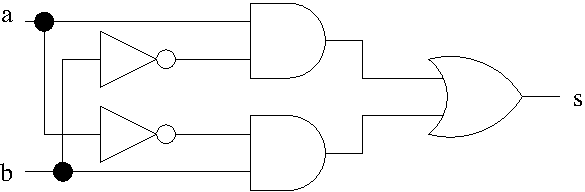
\includegraphics[width=6cm]{ex1.pdf}\end{minipage}
	\hspace*{3mm}
	\begin{py}{8cm}
	\begin{verbatim}
	>>> s = (a and not b) or (b and not a)
	\end{verbatim}
	\end{py}

	\item \begin{minipage}{6cm}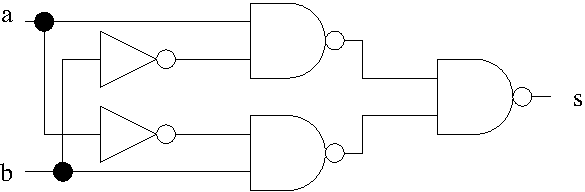
\includegraphics[width=6cm]{ex2.pdf}\end{minipage}
	\hspace*{3mm}
	\begin{py}{8cm}
	\begin{verbatim}
	>>> s = not (not (a and not b) 
	...          and 
	...          not (b and not a))
	\end{verbatim}
	\end{py}

	\item  \begin{minipage}{6cm}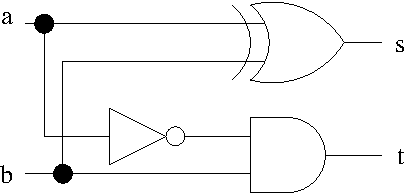
\includegraphics[width=4.5cm]{demiSous.pdf}\end{minipage}
	\hspace*{3mm}
	\begin{py}{8cm}
	\begin{verbatim}
	>>> s = (a and not b) or (not a and b)
	>>> t = (not a) and b
	\end{verbatim}
	\end{py}

	\item \begin{minipage}{6cm}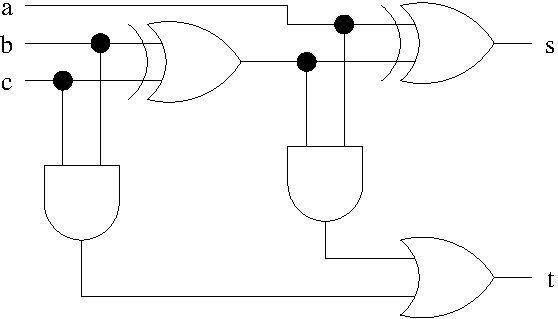
\includegraphics[width=5cm]{add3.pdf}\end{minipage}
	\hspace*{3mm}
	\begin{py}{8cm}
	\begin{verbatim}
	>>> s = (a != (b != c))
	>>> t = (b and c) or (a and (b != c))
	\end{verbatim}
	\end{py}

	\item \begin{minipage}{6cm}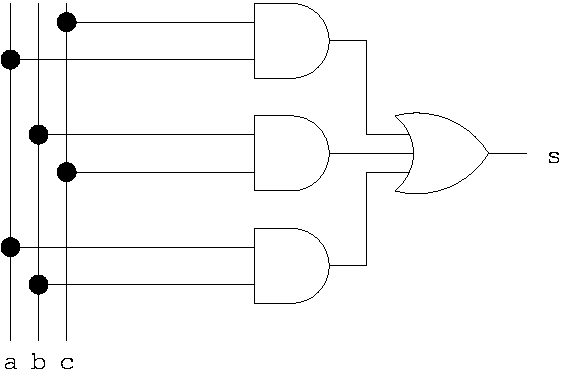
\includegraphics[width=6cm]{majorite.pdf}\end{minipage}
	\hspace*{3mm}
	\begin{py}{8cm}
	\begin{verbatim}
	>>> s = (a and c) or (b and c) or (a and b)
	\end{verbatim}
	\end{py}

	\item \begin{minipage}{6cm}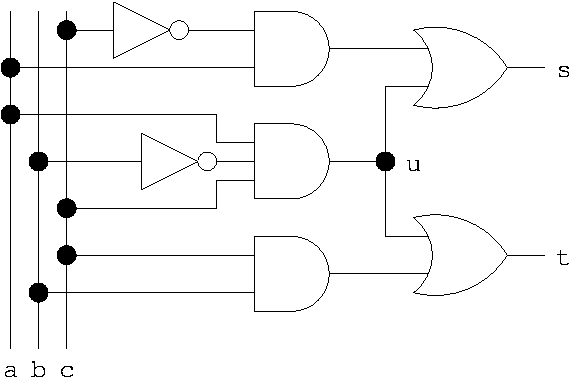
\includegraphics[width=6cm]{circuit.pdf}\end{minipage}
	\hspace*{3mm}
	\begin{py}{8cm}
	\begin{verbatim}
	>>> u = a and (not b) and c
	>>> s = (a and not c) or u
	>>> t = (b and c) or u
	\end{verbatim}
	\end{py}

	\item \begin{minipage}{6cm}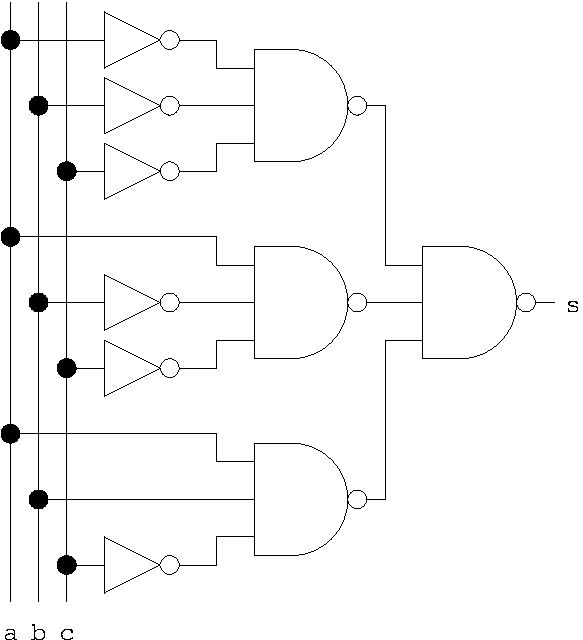
\includegraphics[width=5.5cm]{f3.pdf}\end{minipage}
	\hspace*{3mm}
	\begin{py}{8cm}
	\begin{verbatim}
	>>> s = not (not (not a and not b and not c)
	...          and
	...          not (a and not b and not c)
	...          and
	...          not (a and b and not c))
	\end{verbatim}
	\end{py}

	$$$$
	
	\item \begin{minipage}{6cm}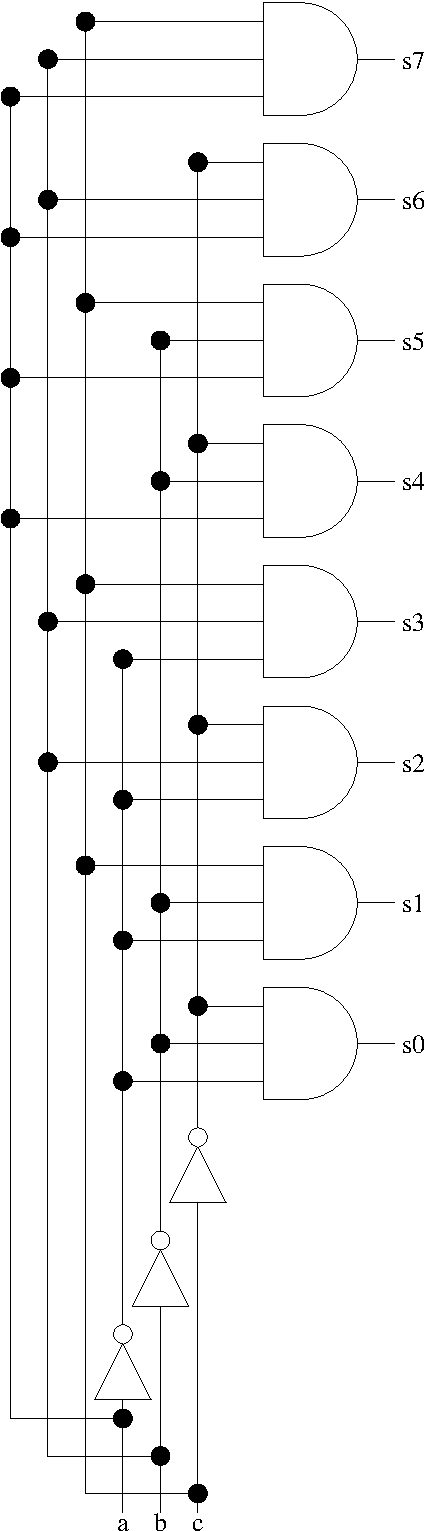
\includegraphics[width=4.5cm]{decodeur.pdf}\end{minipage}
	\hspace*{3mm}
	\begin{py}{8cm}
	\begin{verbatim}
	>>> s7 = a and b and c
	>>> s6 = a and b and not c
	>>> s5 = a and not b and c
	>>> s4 = a and not b and not c
	>>> s3 = not a and b and c
	>>> s2 = not a and b and not c
	>>> s1 = not a and not b and c
	>>> s0 = not a and not b and not c
	\end{verbatim}
	\end{py}
	\end{enumerate}

\item[TD \ref{td:reciproque} :] Alternative simple et test simple.\\
	Il suffit que {\tt blocIf} modifie la condition de telle
	manière qu'elle devienne fausse.
	
	\begin{py}{5cm}
	\begin{verbatim}
	>>> x = - 1
	>>> if x < 0 : x = 3
	... 
	>>> if x >= 0 : x = -1
	... 
	>>> print(x)
	-1
	\end{verbatim}
	\end{py}
	\hfill
	\begin{py}{5cm}
	\begin{verbatim}
	>>> x = -1
	>>> if x < 0 : x = 3
	... else: x = -1
	... 
	>>> print(x)
	3
	\end{verbatim}
	\end{py}
	
\item[TD \ref{td:trinome} :] Racines du trinome.\index[algo]{racines du trinome}

	\begin{py}{12cm}
	\begin{verbatim}
	>>> delta = b*b - 4*a*c
	>>> if delta > 0 :
	...   x1 = (-b - sqrt(delta))/(2*a)
	...   x2 = (-b + sqrt(delta))/(2*a)
	...   n = 2
	... elif delta == 0 :
	...   x1 = x2 = -b/(2*a)
	...   n = 1
	... else : n = 0
	... 
	\end{verbatim}
	\end{py}

\item[TD \ref{td:seq3} :] Séquences de tests.
	\begin{enumerate}
	\item 

		\begin{py}{12cm}
		\begin{verbatim}
		>>> x
		3
		\end{verbatim}
		\end{py}

	\item 

		\begin{py}{12cm}
		\begin{verbatim}
		>>> y
		1
		\end{verbatim}
		\end{py}

	\item 

		\begin{py}{12cm}
		\begin{verbatim}
		>>> y
		1
		\end{verbatim}
		\end{py}

	\item 

		\begin{py}{12cm}
		\begin{verbatim}
		>>> ok
		1
		\end{verbatim}
		\end{py}

	\item 

		\begin{py}{12cm}
		\begin{verbatim}
		>>> y
		5
		\end{verbatim}
		\end{py}

	\end{enumerate}

\item[TD \ref{td:racine} :] Racine carrée entière.\index[algo]{racine carrée entière}

	\begin{py}{12cm}
	\begin{verbatim}
	>>> n = 8
	>>> r = 0
	>>> while (r+1)**2 <= n :
	...   r = r + 1
	... 
	\end{verbatim}
	\end{py}

\item[TD \ref{td:iterations} :] Exécutions d'instructions itératives.\\
	\begin{minipage}[t]{7.5cm}
	\begin{enumerate}
	\item L'algorithme demande d'entrer un nombre au clavier tant que ce nombre
		n'est pas égal à 33

	\begin{py}{12cm}
	\begin{verbatim}
	...
	entrer un nombre : 2
	entrer un nombre : 0
	entrer un nombre : 'fin'
	entrer un nombre : 3.14
	entrer un nombre : 33
	>>> 
	\end{verbatim}
	\end{py}

	\item L'algorithme demande d'entrer un nombre au clavier tant que ce nombre
		n'appartient pas à l'intervalle $]0;5]$.

	\begin{py}{12cm}
	\begin{verbatim}
	...  
	entrer un nombre : 0
	entrer un nombre : 6
	entrer un nombre : 3.14
	>>> 
	\end{verbatim}
	\end{py}

	\item L'algorithme calcule la somme des 5 nombres entrés au clavier.

	\begin{py}{12cm}
	\begin{verbatim}
	... 
	entrer un nombre : 1
	entrer un nombre : 3
	entrer un nombre : 2
	entrer un nombre : 3
	entrer un nombre : 6
	>>> s
	15
	\end{verbatim}
	\end{py}
	\end{enumerate}
	\end{minipage}
	\hfill
	\begin{minipage}[t]{7.5cm}
	\begin{enumerate}\setcounter{enumi}{3}
	\item L'algorithme affiche des étoiles ({\tt *}) selon la disposition
		suivante :

	\begin{py}{12cm}
	\begin{verbatim}
	... 

	*
	* *
	* * *
	* * * *
	* * * * *
	* * * * * *
	* * * * * * *
	* * * * * * * *
	* * * * * * * * *
	>>> 
	\end{verbatim}
	\end{py}

	\item L'algorithme affiche des étoiles ({\tt *}) selon la disposition
		suivante :

	\begin{py}{12cm}
	\begin{verbatim}
	... 
	* * * * * * * * * *
	* * * * * * * * *
	* * * * * * * *
	* * * * * * *
	* * * * * *
	* * * * *
	* * * *
	* * *
	* *
	*
	>>> 
	\end{verbatim}
	\end{py}
	\end{enumerate}
	\end{minipage}

	\begin{minipage}[t]{7.5cm}
	\begin{enumerate}\setcounter{enumi}{5}
	
	\item L'algorithme affiche les tables de multiplication de 0 à 9.

	\begin{py}{12cm}
	\begin{verbatim}
	... 
	1 x 0  =  0
	1 x 1  =  1
	1 x 2  =  2
	1 x 3  =  3
	1 x 4  =  4
	1 x 5  =  5
	1 x 6  =  6
	1 x 7  =  7
	1 x 8  =  8
	1 x 9  =  9
	1 x 10  =  10

	2 x 0  =  0
	2 x 1  =  2
	2 x 2  =  4
	2 x 3  =  6
	2 x 4  =  8
	2 x 5  =  10
	2 x 6  =  12
	2 x 7  =  14
	2 x 8  =  16
	2 x 9  =  18
	2 x 10  =  20

	3 x 0  =  0
	3 x 1  =  3
	3 x 2  =  6
	3 x 3  =  9
	3 x 4  =  12
	3 x 5  =  15
	3 x 6  =  18
	etc...
	\end{verbatim}
	\end{py}
	\end{enumerate}
	\end{minipage}
	\hfill
	\begin{minipage}[t]{7.5cm}
	\begin{enumerate}\setcounter{enumi}{6}
	
	\item L'algorithme affiche le triangle de Pascal jusqu'à l'ordre $n = 9$.\index[algo]{triangle de {{\sc Pascal}}}\\
		Il s'agit des coefficients du binôme $\displaystyle (x+y)^n = \sum_{p=0}^n \frac{n!}{p!(n-p)!}x^{n-p}y^{p}$


	\begin{py}{12cm}
	\begin{verbatim}
	...
	1
	1 1
	1 2 1
	1 3 3 1
	1 4 6 4 1
	1 5 10 10 5 1
	1 6 15 20 15 6 1
	1 7 21 35 35 21 7 1
	1 8 28 56 70 56 28 8 1
	1 9 36 84 126 126 84 36 9 1
	>>> 
	\end{verbatim}
	\end{py}

	 \item  L'algorithme affiche les 15 premiers nombres de la suite de
 		Fibonacci : $u_0=1$, $u_1=1$, $u_n = u_{n-1} + u_{n-2}$.\index[algo]{nombres de {{\sc Fibonacci}}}

	\begin{py}{12cm}
	\begin{verbatim}
	... 
	1 1 2 3 5 8 13 21 34 55 89 144 233 377 610
	>>> 
	\end{verbatim}
	\end{py}

	\item L'algorithme affiche les chiffres de la représentation de $n$ sur $k$ bits maximum
		en base $b$ (du plus petit chiffre au plus grand). Après exécution, la valeur de $s$
		est simplement celle de $n$ : on vérifie ainsi que la conversion en base $b$ est correcte.
		Dans l'exemple ($n=23$, $b=2$ et $k=8$), la valeur de $s$ est 
		$1\cdot 2^0 + 1\cdot 2^1 + 1\cdot 2^2 + 0\cdot 2^3 + 1\cdot 2^4 = 23 = n$.
		\index[algo]{codage en base $b$}

	\begin{py}{12cm}
	\begin{verbatim}
	... 
	1 1 1 0 1
	>>> s
	23
	\end{verbatim}
	\end{py}
	\end{enumerate}
	\end{minipage}


\item[TD \ref{td:geometrieInstruc} :] Figures géométriques.
	\begin{enumerate}
	\item Périmètre $p$ et surface $s$ d'un rectangle de longueur
		$L$ et de largeur $l$

		\begin{py}{12cm}
		\begin{verbatim}
		>>> p = 2*(L+l)
		>>> s = L*l
		\end{verbatim}
		\end{py}

	\item Périmètre $p$ et surface $s$ d'un cercle de rayon $r$

		\begin{py}{12cm}
		\begin{verbatim}
		>>> p = 2*pi*r
		>>> s = pi*r*r
		\end{verbatim}
		\end{py}

	\item Surface latérale $s$ et volume $v$ d'un cylindre de rayon $r$
		et de hauteur $h$

		\begin{py}{12cm}
		\begin{verbatim}
		>>> s = 2*pi*r*h
		>>> v = pi*r*r*h
		\end{verbatim}
		\end{py}

	\item Surface $s$ et volume $v$ d'une sphère de rayon $r$

		\begin{py}{12cm}
		\begin{verbatim}
		>>> s = 4*pi*r*r
		>>> v = 4*pi*r*r*r/3  # v = 4*pi*r**3/3
		\end{verbatim}
		\end{py}
	\end{enumerate}

\item[TD \ref{td:suites} :] Suites numériques.\index[algo]{suites numériques}
	\begin{enumerate}
	\item Somme $s = \sum_0^n u_k$ des $n$ premiers termes d'une suite 
		arithmétique $u_k = a + r\cdot k$

	$$\displaystyle s = \sum_{k=0}^n (a + bk) = a(n+1) + b\sum_{k=1}^n k$$ 
	avec
	$\displaystyle S = \sum_{k=1}^n k = (1 + 2 + 3 + \cdots + n) =
	\frac{n(n+1)}{2}$
	$$\displaystyle\begin{array}[t]{rcccccccccccc}
	S &=& 1 &+& 2 &+& 3 &+& \cdots &+& n & & \\
	S &=& n &+& n-1 &+& n-2 &+& \cdots &+& 1 & & \\
	\hline
	2S &=& (n+1) &+& (n+1) &+& (n+1)&+& \cdots &+& (n+1) &=& n(n+1)\\
	\end{array}$$
	

	\begin{py}{6cm}
	Version constante :
	\begin{verbatim}
	>>> s = a*(n+1) + b*n*(n+1)/2
	\end{verbatim}
	\end{py}
	\hfill
	\begin{py}{6cm}
	Version itérative :
	\begin{verbatim}
	>>> s = 0
	>>> for i in range(n+1) :
	...   s = s + a + b*i
	... 
	\end{verbatim}
	\end{py}

	\item Somme $s = \sum_0^n u_k$ des $n$ premiers termes d'une suite 
		géométrique $u_k = a\cdot b^k$

	$$\displaystyle s = \sum_{k=0}^n ab^k = a\sum_{k=0}^n b^k$$

	où l'expression $\displaystyle N = (b^0+b^1+b^2+\cdots+b^n)$ peut être vue comme le nombre 
	$\displaystyle (111\cdots 1)_b$ en base $b$. Or en base $b$, le nombre $\displaystyle (b-1)(b^0+b^1+b^2+\cdots+b^n)$
	est le nombre immédiatement inférieur à $\displaystyle b^{n+1}$, soit $\displaystyle (b-1)N =
	b^{n+1}-1$.\\
	Exemple en base $b=10$ : $999_{10} = 9(10^0 + 10^1 + 10^2) = 10^3 - 1$
	$$\displaystyle S = \sum_{k=0}^n b^k = (b^0+b^1+b^2+\cdots+b^n) = \frac{b^{n+1}-1}{b-1}$$

	\begin{py}{6cm}
	Version constante :
	\begin{verbatim}
	>>> s = a*(b**(n+1) - 1)/(b-1)
	\end{verbatim}
	\end{py}
	\begin{py}{6cm}
	Version itérative :
	\begin{verbatim}
	>>> s = 0
	>>> for i in range(n+1) :
	...   s = s + a*b**i
	... 
	\end{verbatim}
	\end{py}
	\end{enumerate}
	
\item[TD \ref{td:vecteurs} :] Calcul vectoriel.\index[algo]{calcul vectoriel}
	\begin{enumerate}
	\item Module $r$ et cosinus directeurs $a$, $b$ et $c$
		d'un vecteur de composantes $(x,y,z)$

		\begin{py}{12cm}
		\begin{verbatim}
		>>> r = sqrt(x*x + y*y + z*z)
		>>> a1 = x/r
		>>> a2 = y/r
		>>> a3 = z/r
		\end{verbatim}
		\end{py}

	\item Le produit scalaire $p = \vec{a}\cdot\vec{b}$ de 2 vecteurs $\vec{a}$ et $\vec{b}$ est défini par
		$\displaystyle p = \sum_i a_ib_i$.

		\begin{py}{12cm}
		\begin{verbatim}
		>>> p = x1*x2 + y1*y2 + z1*z2
		\end{verbatim}
		\end{py}

	\item Le produit vectoriel $\vec{c} = \vec{a} \times \vec{b}$ de 2 vecteurs $\vec{a}$ et $\vec{b}$ 
		est un vecteur perpendiculaire au plan du parallélogramme défini par $\vec{a}$ et $\vec{b}$
		et dont la longueur est égale à la surface de ce parallélogramme.

		\begin{py}{12cm}
		\begin{verbatim}
		>>> x3 = y1*z2 - z1*y2
		>>> y3 = z1*x2 - x1*z2
		>>> z3 = x1*y2 - y1*x2
		\end{verbatim}
		\end{py}

	\item Le produit mixte $v = (\vec{a}\times\vec{b})\cdot \vec{c}$ de 3 vecteurs $\vec{a}$, 
		$\vec{b}$ et $\vec{c}$ représente le volume du parallélépipède construit sur ces 3 vecteurs.

		\begin{py}{12cm}
		\begin{verbatim}
		>>> v = (y1*z2 - z1*y2)*x3 + (z1*x2 - x1*z2)*y3 + (x1*y2 - y1*x2)*z3
		\end{verbatim}
		\end{py}
	\end{enumerate}

\item[TD \ref{td:photocopie} :] Prix d'une photocopie.\\
	\begin{py}{12cm}
	\begin{verbatim}
	>>> if n > 30 : s = 10*0.1 + 20*0.09 + (n-30)*0.08
	... elif n > 10 : s = 10*0.1 + (n - 10)*0.09
	... else : s = n*0.1
	...
	\end{verbatim}
	\end{py}

\item[TD \ref{td:impot} :] Calcul des impôts.\\
	\begin{py}{12cm}
	\begin{verbatim}
	>>> if a > 18 :
	...   if s == 'm' : print('impôt')
	...   elif a < 35 : print('impôt')
	...   else : print("pas d'impôt")
	... else : print("pas d'impôt")
	...
	\end{verbatim}
	\end{py}

\item[TD \ref{td:dev} :] Développements limités.\index[algo]{développements limités}\\
	Pour chacun des algorithmes proposés, on pourra vérifier la valeur
	obtenue avec celle de la fonction correspondante dans le module {\tt math} 
	de \python.

	\begin{py}{12cm}
	\begin{verbatim}
	>>> from math import *
	\end{verbatim}
	\end{py}

	\begin{enumerate}
	\item $\displaystyle y = \sinh(x) \approx \sum_{k=0}^{n} \frac{x^{2k+1}}{(2k+1)!} = 
		x + \frac{x^3}{6} + \frac{x^5}{120} + \ldots + \frac{x^{2n+1}}{(2n+1)!}$\\\mbox{}\hfill
		avec
		$\displaystyle u_{k+1} = \frac{x^{2(k+1)+1}}{(2(k+1)+1)!} = \frac{x^2}{(2k+2)(2k+3)}\cdot\frac{x^{2k+1}}{(2k+1)!} 
		= \frac{x^2}{(2k+2)(2k+3)}u_k$

		\begin{py}{12cm}
		\begin{verbatim}
		>>> k = 0
		>>> u = x
		>>> y = u
		>>> s = 1.e-6
		>>> while fabs(u) > s :
		...   u = u*x*x/((2*k+2)*(2*k+3))
		...   y = y + u
		...   k = k + 1
		... 
		\end{verbatim}
		\end{py}

	\item $\displaystyle y = \cosh(x) \approx \sum_{k=0}^{n} \frac{x^{2k}}{(2k)!} = 
		1 + \frac{x^2}{2} + \frac{x^4}{24} + \ldots + \frac{x^{2n}}{(2n)!}$\\\mbox{}\hfill
		avec
		$\displaystyle u_{k+1} = \frac{x^{2(k+1)}}{(2(k+1))!} = \frac{x^2}{(2k+1)(2k+2)}\cdot\frac{x^{2k}}{(2k)!} 
		= \frac{x^2}{(2k+1)(2k+2)}u_k$

		\begin{py}{12cm}
		\begin{verbatim}
		>>> k = 0
		>>> u = 1.
		>>> y = u
		>>> s = 1.e-6
		>>> while fabs(u) > s :
		...   u = u*x*x/((2*k+1)*(2*k+2))
		...   y = y + u
		...   k = k + 1
		... 
		\end{verbatim}
		\end{py}

	\item $\displaystyle y = \cos(x) \approx \sum_{k=0}^{n} (-1)^k\frac{x^{2k}}{(2k)!} = 
		1 - \frac{x^2}{2} + \frac{x^4}{24} + \ldots + (-1)^n\frac{x^{2n}}{(2n)!}$\\\mbox{}\hfill
		avec
		$\displaystyle u_{k+1} = (-1)^k\frac{x^{2(k+1)}}{(2(k+1))!} = \frac{-x^2}{(2k+1)(2k+2)}\cdot(-1)^k\frac{x^{2k}}{(2k)!}
		= \frac{-x^2}{(2k+1)(2k+2)}u_k$

		\begin{py}{12cm}
		\begin{verbatim}
		>>> k = 0
		>>> u = 1.
		>>> y = u
		>>> s = 1.e-6
		>>> while fabs(u) > s :
		...   u = -u*x*x/((2*k+1)*(2*k+2))
		...   y = y + u
		...   k = k + 1
		... 
		\end{verbatim}
		\end{py}

	\item $\displaystyle y = \log(1+x) \approx \sum_{k=0}^{n} (-1)^k\frac{x^{k+1}}{k+1} = 
		x - \frac{x^2}{2} + \frac{x^3}{3} + \ldots + (-1)^n\frac{x^{n+1}}{n+1}$\ , 
		pour $-1 < x < 1$\\\mbox{}\hfill
		avec
		$\displaystyle u_{k+1} = (-1)^k\frac{x^{(k+1)+1}}{(k+1)+1} = -x\frac{k+1}{k+2}\cdot(-1)^k\frac{x^{k+1}}{k+1}
		= -x\frac{k+1}{k+2}u_k$

		\begin{py}{12cm}
		\begin{verbatim}
		>>> if fabs(x) < 1 :
		...   k = 0
		...   u = x
		...   y = u
		...   s = 1.e-6
		...   while fabs(u) > s :
		...     u = -u*x*(k+1)/(k+2)
		...     y = y + u
		...     k = k + 1
		... 
		\end{verbatim}
		\end{py}

	\item $\displaystyle y = \arctan(x) \approx \sum_{k=0}^{n} (-1)^k \frac{x^{2k+1}}{(2k+1)} = 
		x - \frac{x^3}{3} + \frac{x^5}{5} + \ldots + (-1)^n \frac{x^{2n+1}}{(2n+1)}$\ , 
		pour $-1 < x < 1$\\\mbox{}\hfill
		avec
		$\displaystyle u_{k+1} = (-1)^k \frac{x^{2(k+1)+1}}{(2(k+1)+1)} = -x^2\frac{2k+1}{2k+3}\cdot(-1)^k \frac{x^{2k+1}}{(2k+1)}
		= -x^2\frac{2k+1}{2k+3}u_k$

		\begin{py}{12cm}
		\begin{verbatim}
		>>> if fabs(x) < 1 :
		...   k = 0
		...   u = x
		...   y = u
		...   s = 1.e-6
		...   while fabs(u) > s :
		...     u = -u*x*x*(2*k+1)/(2*k+3)
		...     y = y + u
		...     k = k + 1
		... 
		\end{verbatim}
		\end{py}

	\end{enumerate}

\item[TD \ref{td:tablesVerite} :] Tables de vérité.\index[algo]{tables de vérité}

	\begin{minipage}[t]{7.5cm}
	\begin{enumerate}
	\item
	
	\begin{py}{12cm}
	\begin{verbatim}
	>>> for a in [0,1] :
	...   for b in [0,1] :
	...     for c in [0,1] :
	...       s = (a and not b) or 
	...           (b and not a)
	...       print(a, b, c, s)
	... 
	0 0 0 0
	0 0 1 0
	0 1 0 1
	0 1 1 1
	1 0 0 1
	1 0 1 1
	1 1 0 0
	1 1 1 0
	\end{verbatim}
	\end{py}

	\item
	
	\begin{py}{12cm}
	\begin{verbatim}
	>>> for a in [0,1] :
	...   for b in [0,1] :
	...     s = not (not (a and not b) 
	...         and 
	...         not (b and not a))
	...     print(a, b, s)
	... 
	0 0 0
	0 1 1
	1 0 1
	1 1 0
	\end{verbatim}
	\end{py}
	\end{enumerate}
	\end{minipage}
	\hfill
	\begin{minipage}[t]{7.5cm}
	\begin{enumerate}\setcounter{enumi}{2}
	\item
	
	\begin{py}{12cm}
	\begin{verbatim}
	>>> for a in [0,1] :
	...   for b in [0,1] :
	...     s = (a and not b) or (not a and b)
	...     t = (not a) and b
	...     print(a, b, s, t)
	... 
	0 0 0 0
	0 1 1 1
	1 0 1 0
	1 1 0 0
	\end{verbatim}
	\end{py}

	\item
	
	\begin{py}{12cm}
	\begin{verbatim}
	>>> for a in [0,1] :
	...   for b in [0,1] :
	...     for c in [0,1] :
	...       s = (a != (b != c))
	...       t = (b and c) or (a and (b != c))
	...       print(a, b, c, s, t)
	...
	0 0 0 0 0
	0 0 1 1 0
	0 1 0 1 0
	0 1 1 0 1
	1 0 0 1 0
	1 0 1 0 1
	1 1 0 0 1
	1 1 1 1 1
	\end{verbatim}
	\end{py}
	\end{enumerate}
	\end{minipage}

	\begin{minipage}[t]{7.5cm}
	\begin{enumerate}\setcounter{enumi}{4}
	\item
	
	\begin{py}{12cm}
	\begin{verbatim}
	>>> for a in [0,1] :
	...   for b in [0,1] :
	...     for c in [0,1] :
	...       s = not (not (a and b) and 
	...           not (a and c) and 
	...           not (b and c))
	...       print(a, b, c, s)
	... 
	0 0 0 0
	0 0 1 0
	0 1 0 0
	0 1 1 1
	1 0 0 0
	1 0 1 1
	1 1 0 1
	1 1 1 1
	\end{verbatim}
	\end{py}

	\item
	
	\begin{py}{12cm}
	\begin{verbatim}
	>>> for a in [0,1] :
	...   for b in [0,1] :
	...     for c in [0,1] :
	...       s = not (not (not a and 
	...                     not b and not c) and 
	...           not (a and not b and 
	...                not c) and 
	...           not (a and b and not c))
	...       print(a, b, c, s)
	... 
	0 0 0 1
	0 0 1 0
	0 1 0 0
	0 1 1 0
	1 0 0 1
	1 0 1 0
	1 1 0 1
	1 1 1 0
	\end{verbatim}
	\end{py}
	\end{enumerate}
	\end{minipage}
	\hfill
	\begin{minipage}[t]{7.5cm}
	\begin{enumerate}\setcounter{enumi}{6}
	\item
	
	\begin{py}{12cm}
	\begin{verbatim}
	>>> for a in [0,1] :
	...   for b in [0,1] :
	...     for c in [0,1] :
	...       u = (b and not c) or (not b and c)
	...       s = (a and not u) or (not a and u)
	...       t = (b and c) or (a and u)
	...       print(a, b, c, u, s, t)
	... 
	0 0 0 0 0 0
	0 0 1 1 1 0
	0 1 0 1 1 0
	0 1 1 0 0 1
	1 0 0 0 1 0
	1 0 1 1 0 1
	1 1 0 1 0 1
	1 1 1 0 1 1
	\end{verbatim}
	\end{py}

	\item
	
	\begin{py}{12cm}
	\begin{verbatim}
	>>> for a in [0,1] :
	...   for b in [0,1] :
	...     for c in [0,1] :
	...       s7 = a and b and c
	...       s6 = a and b and not c
	...       s5 = a and not b and c
	...       s4 = a and not b and not c
	...       s3 = not a and b and c
	...       s2 = not a and b and not c
	...       s1 = not a and not b and c
	...       s0 = not a and not b and not c
	...       print(a, b, c, s0, s1, s2, s3, s4, s5, s6, s7)
	... 
	0 0 0 1 0 0 0 0 0 0 0
	0 0 1 0 1 0 0 0 0 0 0
	0 1 0 0 0 1 0 0 0 0 0
	0 1 1 0 0 0 1 0 0 0 0
	1 0 0 0 0 0 0 1 0 0 0
	1 0 1 0 0 0 0 0 1 0 0
	1 1 0 0 0 0 0 0 0 1 0
	1 1 1 0 0 0 0 0 0 0 1
	\end{verbatim}
	\end{py}
	\end{enumerate}
	\end{minipage}

\item[TD \ref{td:dessins} :] Dessins géométriques.
	\begin{enumerate}
	\item Une étoile à 5 branches
	\item Un losange
	\end{enumerate}

\item[TD \ref{td:assurance} :] Police d'assurance.\\
	Il s'agit en fait d'une assurance à points ($p$) qui
	dépend de l'âge $a$ du conducteur, de l'ancienneté $d$ 
	du permis, du nombre $n$ d'accidents et du nombre $r$ d'années
	en tant qu'assuré fidèle.
	
	\begin{py}{12cm}
	\begin{verbatim}
	>>> p = 0
	>>> if a < 25 : p = p + 1            # jeune
	... 
	>>> if d < 2 : p = p + 1             # jeune conducteur
	... 
	>>> p = p + n                        # accidents
	>>> 
	>>> if p < 3 and r > 1 : p = p - 1   # fidélité
	... 
	>>> if p == -1 : print('tarif A')
	... elif p == 0 : print('tarif B')
	... elif p == 1 : print('tarif C')
	... elif p == 2 : print('tarif D')
	... else : print('refus d'assurer') 
	...
	\end{verbatim}
	\end{py}

\item[TD \ref{td:zero} :] Zéro d'une fonction.\index[algo]{zéro d'une fonction}
	\begin{enumerate}
	\item Méthode par dichotomie

		\begin{py}{12cm}
		\begin{verbatim}
		>>> x1 = 1.
		>>> x2 = 3.
		>>> x = (x1 + x2)/2.
		>>> s = 1.e-9
		>>> f = cos
		>>> while (x2 - x1) > s :
		...   if f(x1)*f(x) < 0 : x2 = x
		...   else : x1 = x
		...   x = (x1 + x2)/2. 
		>>> x, cos(x)
		(1.5707963271997869, -4.048902822446996e-10)
		\end{verbatim}
		\end{py}

	\item Méthode des tangentes

		\begin{py}{12cm}
		\begin{verbatim}
		>>> x1 = 1.
		>>> x2 = 2.
		>>> s = 1.e-9
		>>> f = cos
		>>> df = sin
		>>> x = x2 - f(x2)/(-df(x2))
		>>> while fabs(x-x2) > s :
		...   x2 = x
		...   x = x - f(x)/(-df(x))
		...
		>>> x, cos(x)
		(1.5707963267948966, 6.1230317691118863e-17)
		\end{verbatim}
		\end{py}

	\item Méthode des sécantes

		\begin{py}{12cm}
		\begin{verbatim}
		>>> x1 = 1.
		>>> x2 = 2.
		>>> s = 1.e-9
		>>> f = cos
		>>> df = (f(x2)-f(x1))/(x2-x1)
		>>> x = x2 - f(x2)/df
		>>> while fabs(x-x2) > s :
		...   x2 = x
		...   df = (f(x2)-f(x1))/(x2-x1)
		...   x = x - f(x)/df
		...
		>>> x, cos(x)
		(1.570796326805755, -1.085836403972619e-11)
		\end{verbatim}
		\end{py}

	\item Méthode des cordes

		\begin{py}{12cm}
		\begin{verbatim}
		>>> x1 = 1.
		>>> x2 = 3.
		>>> x = (x2*f(x1) - x1*f(x2))/(f(x1)-f(x2))
		>>> s = 1.e-9
		>>> f = cos
		>>> while (x2-x1) > s :
		...   if f(x1)*f(x) < 0 : x2 = x
		...   else : x1 = x
		...   x = (x2*f(x1) - x1*f(x2))/(f(x1)-f(x2))
		... 
		>>> x, cos(x)
		(1.5707963267948966, 6.1230317691118863e-17)
		\end{verbatim}
		\end{py}

	\end{enumerate}

\end{description}


%-------------------------------------------------------------------------
\newpage
\setlength{\textwidth}{16cm}
\setlength{\linewidth}{16cm}
\setlength{\textheight}{16cm}
\setlength{\marginparwidth}{8cm}
\setlength{\marginparsep}{1cm}
\setlength{\oddsidemargin}{0cm}
\setlength{\evensidemargin}{+8cm}
\setlength{\topmargin}{-0.75cm}

\section{Annexes}
%-------------------------------------------------------------------------

%-------------------------------------------------------------------------
\subsection{Instructions {\sc Logo}}\label{logo}\index{langage!{{\sc Logo}}}
%-------------------------------------------------------------------------
\begin{quote}\scriptsize\em 
{\em Logo is the name for a philosophy of education and 
a continually evolving family of programming languages that aid in its realization
(Harold Abelson, Apple Logo, 1982).}
This statement sums up two fundamental aspects of Logo and puts them in the proper order. 
The Logo programming environments that have been developed over the past 28 years are 
rooted in constructivist educational philosophy, and are designed to support constructive 
learning. [\ldots]
Constructivism views knowledge as being created by learners in their own minds through 
interaction with other people and the world around them. This theory is most closely 
associated with Jean Piaget, the Swiss psychologist, who spent decades studying and 
documenting the learning processes of young children.\\
\mbox{}\hfill {\rm\bf Logo Foundation :} 
\href{http://el.media.mit.edu/logo-foundation}{\tt http\char`://el.media.mit.edu/logo-foundation}
\end{quote}

On suppose connues les procédures de tracés géométriques {\em à la {\sc Logo}} :\vspace*{2mm}

\mbox{}\hspace*{1cm}
\begin{minipage}{\textwidth}\footnotesize
\begin{description}
\item[\tt degrees()] fixe l'unité d'angle en degrés
\item[\tt radians()] fixe l'unité d'angle en radians
\item[\tt reset()] efface l'écran et réinitialise les variables
\item[\tt clear()] efface l'écran
\item[\tt up()] lève le crayon 
\item[\tt down()] abaisse le crayon 
\item[\tt forward(d)] avance d'une distance $d$
\item[\tt backward(d)] recule d'une distance $d$
\item[\tt left(a)] tourne sur la gauche d'un angle $a$
\item[\tt right(a)] tourne sur la droite d'un angle $a$
\item[\tt goto(x,y)] déplace le crayon à la position $(x,y)$
\item[\tt towards(x,y)] oriente vers le point de coordonnées $(x,y)$
\item[\tt setheading(a)] oriente d'un angle $a$ par rapport à l'axe des $x$
\item[\tt position()] donne la position $(x,y)$ du crayon
\item[\tt heading()] donne l'orientation $a$ du déplacement 
\item[\tt circle(r)] trace un cercle de rayon $r$
\item[\tt circle(r,a)] trace un arc de cercle de rayon $r$ et d'angle au sommet $a$.
\end{description}
\end{minipage}

%-------------------------------------------------------------------------
\subsection{Instructions {\sc Python}}\label{python}\index{langage!{{\sc Python}}!instructions}
%-------------------------------------------------------------------------
Les principales instructions {\sc Python} sont listées dans les tableaux
ci-dessous.

\begin{longtable}{|p{5.5cm}|p{9.5cm}|}
\multicolumn{2}{l}{\bf Miscellaneous statements}\\
\hline
\bf Statement & \bf Result \\
\hline
\tt pass & Null statement \\
\hline
\tt del name[, name]* &	Unbind {\tt name}(s) from object \\
\hline
\tt print([s1 [, s2 ]*) & Writes to {\tt sys.stdout}, or to {\tt file\-object} if supplied. 
                                             Puts spaces between arguments {\tt si}. Puts newline at end unless arguments end with {\tt end=} (ie: {\tt end=' '}). 
					     {\tt print} is not required when running interactively, simply typing an expression will print its value, 
					     unless the value is {\tt None}.\\
\hline
\tt input([prompt]) & 	Prints {\tt prompt} if given. Reads input and evaluates it. \\
\hline
\multicolumn{2}{l}{}\\
\multicolumn{2}{l}{\bf Assignment operators}\\
\hline
\bf Operator & \bf Result \\
\hline
\tt a = b 	& Basic assignment - assign object {\tt b} to label {\tt a}\\
\hline
\tt a += b 	& \tt a = a + b 	\\
\tt a -= b 	& \tt a = a - b 	\\
\tt a *= b 	& \tt a = a * b 	\\
\tt a /= b 	& \tt a = a / b 	\\
\tt a //= b 	& \tt a = a // b	\\
\tt a \%= b 	& \tt to a = a \% b	\\
\tt a **= b 	& \tt to a = a ** b	\\
\tt a \&= b 	& \tt a = a \& b	\\
\tt a |= b 	& \tt a = a | b 	\\
\tt a \char`^= b& \tt a = a \char`^\ b 	\\
\tt a >>= b 	& \tt a = a >> b	\\
\tt a <<= b 	& \tt a = a << b	\\
\hline
\multicolumn{2}{l}{}\\
\multicolumn{2}{l}{\bf Control flow statements}\\
\hline
\bf Statement & \bf Result \\
\hline
\tt if condition:\newline
\mbox{}\ \ suite\newline
[elif condition: suite]*\newline
[else:\newline
\mbox{}\ \ suite] & Usual {\tt if/else if/else} statement.\\
\hline
\tt while condition:\newline
\mbox{}\ \ suite\newline
[else:\newline
\mbox{}\ \ suite] & Usual {\tt while} statement. The {\tt else suite} is executed after 
           loop exits, unless the loop is exited with {\tt break}.\\
\hline
\tt for element in sequence:\newline
\mbox{}\ \ suite\newline
[else:\newline
\mbox{}\ \ suite] & Iterates over {\tt sequence}, assigning each element to {\tt element}. 
           Use built-in {\tt range} function to iterate a number of times. 
	   The {\tt else suite} is executed at end unless loop exited with {\tt break}.\\
\hline
\tt break & Immediately exits for or while loop.\\
\tt continue & Immediately does next iteration of for or while loop.\\
\hline
\tt return [result] & Exits from function (or method) and returns {\tt result} 
                     (use a tuple to return more than one value).\\
\hline
\end{longtable}

\noindent{\bf Name space statements}\\
Imported module files must be located in a directory listed in the {\tt path} ({\tt sys.path}).
 
Packages: a package is a name space which maps to a directory including 
module(s) and the special initialization module {\tt \_\_init\_\_.py} (possibly empty).

Packages/directories can be nested. You address a module's symbol via \\
{\tt [package.[package...].module.symbol} .

\begin{longtable}{|p{5.5cm}|p{9.5cm}|}
\hline
\bf Statement & \bf Result \\
\hline
{\tt import module1 [as name1] [, module2]*} 	& Imports modules. 
	Members of module must be referred to by qualifying with {\tt [package.]module} name, e.g.:\newline
	{\tt \mbox{}\ \ import sys; print(sys.argv)\newline
	\mbox{}\ \ import package1.subpackage.module\newline
	\mbox{}\ \ package1.subpackage.module.foo()}\newline
	{\tt module1} renamed as {\tt name1}, if supplied.\\
\hline
{\tt \tt from module import name1 [as othername1][, name2]*} 	& Imports {\tt name}s from module {\tt module} 
	in current namespace, e.g. :\newline
{\tt 
\mbox{}\ \ from sys import argv; print(argv)\newline
\mbox{}\ \ from package1 import module; \newline\mbox{}\ \ module.foo()\newline
\mbox{}\ \ from package1.module import foo; \newline\mbox{}\ \ foo()}\newline
{\tt name1} renamed as {\tt othername1}, if supplied.\\
\hline
{\tt from module import * } 	 & Imports all names in {\tt module}, except those starting with {\tt \_}. \\
\hline
\end{longtable}



